\chapter{Marco teórico}

Este capítulo aborda, de manera breve, rápida y concisa, nociones matemáticas y
fundamentos físicos necesarios para los métodos químico-cuánticos utilizados en
esta tesis. Entre ellos se encuentran métodos de estructura electrónica, como
Hartree-Fock y Teoría de los Funcionales de la Densidad. Además del método IQA,
el cual es utilizado para analizar  la energía de interacción en los EHs
encontrados de diversos cúmulos de agua.

Finalmente, con este marco teórico, se pretende tener una idea general y
concisa de las teorías y postulados bajo los cuales se obtuvieron los
resultados en los que se basan las conclusiones de esta tesis. De la misma
forma, también se dedica un apartado a la presentación de los detalles
computacionales.

\section{Topología}

Para la comprensión de la topología es necesario tomar una pequeña idea de que
es la geometría y de sus límites, como dijo Henrie Poincaré ``{\em ...geometría
es el arte de razonar bien a partir de dibujos mal hechos}''. Esto claro,
únicamente a modo de alegoría. Debido a los diversos tipos de geometría es
usual que este término venga acompañado de algún otro nombre, como geometría
euclidiana, geometría algebraica, geometría hiperbólica, entre otros.

En 1872 Felix Klein, en su proyecto de investigación Erlangen, sugirió que la
geometría no debe definirse a través de los objetos que se están estudiando,
sino por las transformaciones que dejan fijas a los objetos. Tales
transformaciones tienen ancladas propiedades como la congruencia o la
semejanza, a las que se les denomina invariantes,
\color{blue}
  \begin{quote}
    ``{\em geometría es la ciencia que estudia las propiedades de las figuras
    que se preservan bajo las transformaciones de cierto grupo de transformaciones.
    Equivalentemente, es la ciencia que estudia los invariantes de un grupo
    de transformaciones}''.
  \end{quote}
\color{black}
Así, una geometría está determinada por un dominio de acción $X$ (el plano, el
espacio, \&c.), y un grupo de automorfismos $G$ (isometrías, similitudes, \&c.)
que actúa en $X$.

En geometría es necesario también el entendimiento del espacio métrico, esta
noción fue introducida por el matemático Frechét y forma parte fundamental de
muchas las ramas de las matemáticas.  Nociones importantes de la topología
fueron desarrolladas primeramente en espacios métricos y luego trasladadas a
espacio topológicos.

Un espacio métrico es un conjunto en el cual se pueden medir la distancia entre
sus puntos, así como la $proximidad$ de un punto a un conjunto, o de un
conjunto a otro. Una métrica es simplemente la formalización de la noción de
\textit{distancia} ordinaria, como se ve en la siguiente
definición~\cite{sergey}.

{\sc{Definición}}. Sea $\mathrm{X}$ un conjunto no vacío. Una función $\rho :
\mathrm{X} \times\mathrm{X} \rightarrow \mathbb{R}$ se llama \textbf{métrica} o
distancia, si para cualesquiera puntos $x, y, z \in \mathrm{X}$ se satisfaces
los siguientes axiomas:
\begin{enumerate}
\item $\rho (x,y) \ge 0$ y $\rho(x,y)=0$ si y sólo si $x=y$.
\item $\rho (x,y) = \rho (y,x)$.
\item $\rho (x,z) \le \rho (x,y)+\rho(y,z)$\\ (esta desigualdad se conoce como
desigualdad del triángulo).
\end{enumerate}

El par $(\mathrm{X},\rho)$ recibe el nombre de \textbf{espacio métrico}. El
número $\rho(x,y)$ suele llamarse distancia entre los puntos $x$ y $y$.

\subsection{Generalidades topológicas}

Numerosos conceptos surgidos del análisis matemático fueron rápidamente
generalizados a espacios mayores. Varios de ellos han sido aplicados a espacios
que localmente son como $\mathbb{R}^\mathrm{n}$. En esta subsección se abordan
algunos conceptos de como se entendía la geometría y como empezó a tener
diversas ``fallas'' en la resolución de algunos problemas, así como algunos
temas clásicos que sirven dentro de la topología.

Si bien los espacios métricos tienen un sinfín de aplicaciones dentro y fuera
de las matemáticas abstractas, hubo un momento donde la geometría en espacios
métricos no podía dar solución a diversos problemas, uno de los más conocidos
es el planteado en el siglo XVIII sobre los puentes de K\"onigsberg, hoy
Kaliningrado.  Dicho problema enuncia: ?`se puede recorrer la ciudad pasando
una única vez por los 7 puentes de la ciudad? La resolución a este problema fue
dado por uno de los más grandes matemáticos de la historia, Leonhard Euler, en
1736. Dicha solución dio paso al surgimiento de la topología y la teoría de
grafos. En la Figura \ref{fig:grafo} se representan a los puentes como aristas
y a las partes de la ciudad conectadas por puentes como vértices. De forma que,
de existir un camino a través de la ciudad en la que sólo se use una única vez
cada puente, de manera equivalente, habrá un modo de trazar las conexiones
entre los vértices sin repetir el trazo de alguna arista en el grafo. 
%%%%%%%%
\begin{figure}[h]
\centering

	\begin{subfigure}{0.45\linewidth}
	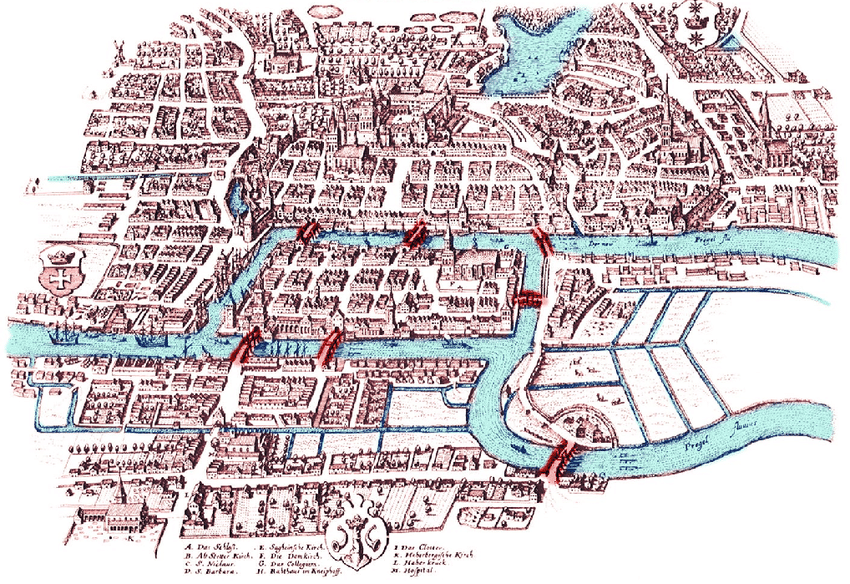
\includegraphics[width=\linewidth]{2/img/puentes}
	\caption{Ilustración del mapa de la Ciudad de K\"onigsberg~\cite{img_puente_k}.}
	\label{fig:mapa}
	\end{subfigure} \hspace{10mm}
%
	\begin{subfigure}{0.38\linewidth}
	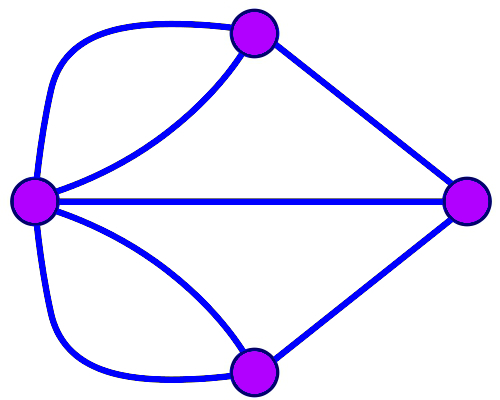
\includegraphics[width=\linewidth]{3/img/grafo_puentes_k}
	\caption{Grafo representativo a los puentes de K\"onigsberg.}
	\label{fig:grafo}
	\end{subfigure}
	
\caption{Ciudad de K\"onigsberg y su grafo correspondiente.}
\label{fig:mapa_grafo}
\end{figure}

La publicación de Euler~\cite{euler1736}, es la primera que hace alusión a una
geometría en donde sólo interesan ciertas propiedades de los objetos, y no su
métrica, como tradicionalmente se hacía. Euler llama a esta nueva manera de ver
a los objetos geométricos como $geometriam$ $situs$, término que hoy se traduce
como topología. El nombre de topología fue dado por Johann Benedict Listing
(alumno de Gauss), al querer hacer destacar el desapego de la geometría y
autonomía de esta nueva rama de las matemáticas~\cite{listing}.
 
Para destacar la diferencia entre la geometría y la $geometriam$ $situs$,
Leonhard Euler, al resolver el problema de los puentes de K\"onigsberg, expone
``{\em además de la geometría que trabaja sobre cantidades, hay otra, que no se
ve afectada por las cantidades. Y por ello cuando se manipula con las
herramientas de la geometría normal, no admite solución}''.

La topología estudia entonces, las propiedades de los cuerpos geométricos que
permanecen invariantes ante transformaciones continuas (también llamadas
suaves), es decir, no cortar o pegar, sólo deformar suavemente~\cite{moderna},
como se muestra en el conocido homeomorfismo de una taza con una dona mostrado
en la Figura \ref{dona_taza}.  Con esta idea, que puede sonar simple, se pueden
abordar temas extremadamente grandes y diversos.
%
\begin{figure}[h]
    \centering
    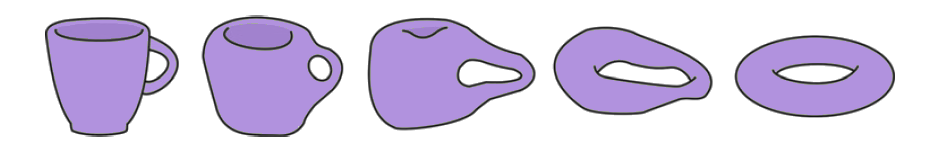
\includegraphics[width=0.55\textwidth]{2/img/dona_taza}
    \caption{Homeomorfismo entre una toro y una taza.}
\label{dona_taza}
\end{figure}

Es necesario entonces ahora hablar de espacios topológicos; llevar a una noción
más abstracta algunos conceptos y propiedades de los espacios métricos a otro
tipo de estructuras matemáticas a las que llamaremos espacios
topológicos~\cite{sergey}.

{\sc{Definición}}. Sea $X$ un conjunto no vacío. Una colección $\tau$ de
subconjuntos de $X$ se llama topología en $X$, si se satisfaces los siguientes
axiomas:
\begin{enumerate}
  \item $\emptyset , X \in \tau$.
  \item Si $\left \{U_{\alpha} \right \}_{\alpha \in A}$ es una familia cualquiera de elementos de $\tau$,
  entonces $\displaystyle\bigcup_{\alpha\in A}{U_\alpha \in\tau}$.
  \item Si $U$ y $V$ son dos elementos de $\tau$, entonces $U \cap V \in \tau$.
\end{enumerate}

Los elementos de $\tau$ reciben el nombre de abiertos de $X$, y el par
$(X,\tau)$ se llama \textbf{espacio topológico}.

\subsection{Importancia de la topología en la ciencia}

Diversas aplicaciones de la topología han surgido con el tiempo: la teoría de
grafos permite dar trayectos óptimos a vuelos o a entregas por paquetería, la
teoría de nudos permite corresponder los anudamientos de las moléculas de ADN a
los existentes en una cuerda, la topología algebraica con el teorema de la bola
peluda permite explicar como es que en todo planeta es imposible que no haya
algún lugar donde no sople el viento, es decir, en algún lugar del planeta no
sopla el viento.

Las aplicaciones actuales de la topología son variadas, por ejemplo, el uso de
la teoría de grafos para colorear mapas, tal como se enuncia en el Teorema de
los Cuatro Colores, ilustrado en la Figura \ref{australia}. El cual afirma que
dado cualquier mapa con regiones continuas, este puede ser coloreado con cuatro
colores diferentes como máximo, de forma que no queden regiones adyacentes con
el mismo color, donde estas regiones adyacentes comparten más de un punto, es
decir existe un borde~\cite{4colores}. Este teorema no es útil sólo para
colorear mapas, la idea de llevar regiones no compatibles a grafos puede
extrapolarse a, por ejemplo, el transporte de objetos en cajas donde diversos
tipos de objetos no son compatibles entre sí o para redes computacionales.

\begin{figure}[h]
  \centering
  \begin{subfigure}[b]{0.28\linewidth}
    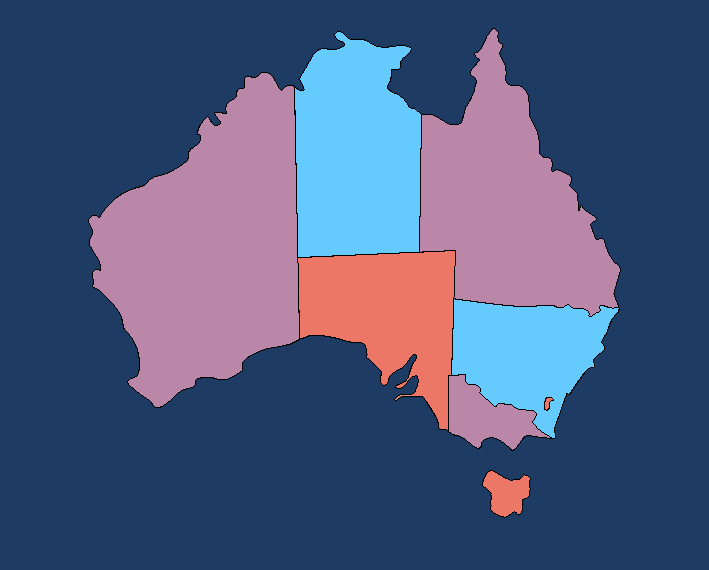
\includegraphics[width=\linewidth]{3/img/4_colors_australia_mapa}
    \caption{Mapa de Australia coloreado con cuatro colores.}
  \end{subfigure}   
    \begin{subfigure}[b]{0.28\linewidth}
    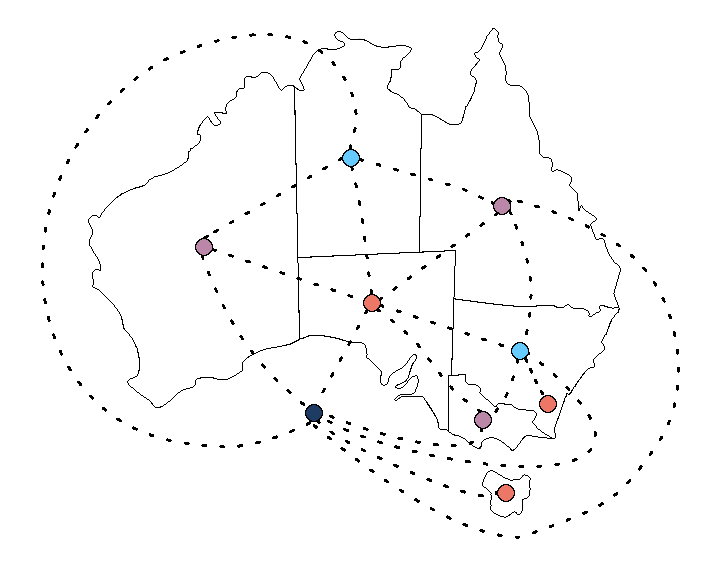
\includegraphics[width=\linewidth]{3/img/4_colors_australia_mapa_y_grafo}
    \caption{Mapa de Australia con el grafo para colorear.}
  \end{subfigure} 
    \begin{subfigure}[b]{0.28\linewidth}
    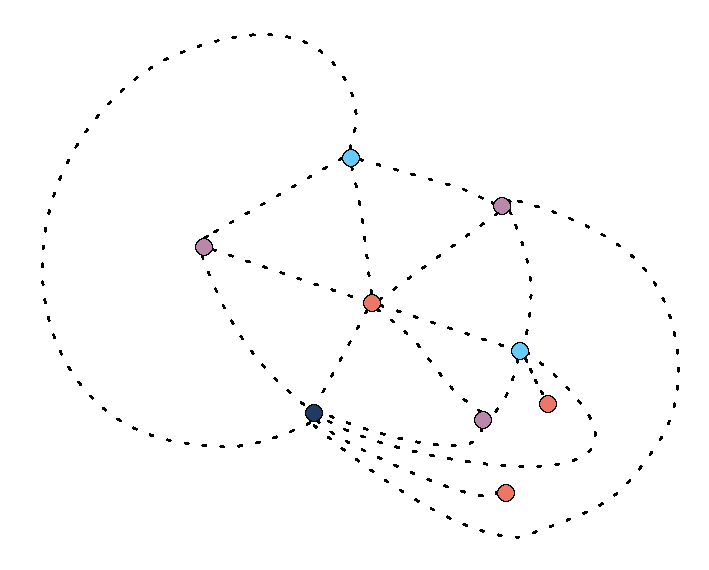
\includegraphics[width=\linewidth]{3/img/4_colors_australia_grafo}
    \caption{Grafo representativo al mapa de Australia.}
  \end{subfigure}
  \caption{Ejemplo del teorema de los cuatro colores.}
  \label{australia}
\end{figure}

Desde el siglo XIX varios matemáticos intentaron demostrar este teorema, con
muchos intentos fallidos e incluso pruebas que terminaron siendo falsas,
llevando a varias personas intentar atacar el problema a través de
contraejemplos (mapas que no podían ser coloreados con cuatro colores sin tener
regiones adyacentes con el mismo color), pero que tampoco condujeron a la
solución. Incluso se llegó a demostrar para cinco colores, es decir, todo mapa
es posible de colorear con un máximo de cinco colores sin regiones adyacentes
del mismo color, pero el de cuatro seguía sin tener demostración o ser
refutado.

No fue hasta 1976 que Kenneth Appel y Wolfgang Haken logran demostrar el
Teorema de los Cuatro Colores, a través de elaborar 1936 mapas  que forman
parte de cualquier contraejemplo al teorema, llegar a esto llevó bastante
trabajo. Pero el verdadero problema era demostrar que todos esos contraejemplos
eran posibles de colorear únicamente con cuatro colores, era tan laborioso que
tuvieron que recurrir a la computación con su fiel IBM 370 ~\cite{50cosas} con
al rededor de \SI{1000}{} horas de cómputo. Esta demostración no estuvo
absuelta de críticas por el uso de una computadora, debido a que podía
``carecer'' de rigor matemático.  Desde ese gran hito del uso de computadoras
en una demostración matemática son cada vez más comunes y aceptados estos
métodos. El uso de computadoras en las diversas ramas de la ciencia es cada vez
más normal, en gran parte debido al crecimiento agigantado del poder de cómputo
y del diseño de algoritmos.

Otra gran rama de la topología, la Teoría de Nudos, aborda la abstracción de la
concepción cotidiana del nudo. Formalmente hablando, un nudo en $\mathbb{R}^3$
es una clase de equivalencia de encajes de la 1-esfera en $\mathbb{R}^3$ o en
la 3-esfera~\cite{nudos}. Es importante marcar que se tiene algunas propiedades
para todo nudo, que ayudan en la distinción entre diferentes tipos de ellos,
los invariantes en nudos son: $i$) la tricoloreabilidad, $ii$) el grupo de un
nudo, que es el grupo fundamental de su complemento, $iii$) el polinomio de
Alexander, $iv$) los invariantes hiperbólicos y $v$) el polinomio de Jones.

La topología no sólo es útil en las matemáticas abstractas, como vimos en
teoría de nudos o en teoría de grafos. Es el caso de la relación entre los
árboles (topológicos) y la química, que fue descubierto en 1874 por Carl
Schorlemmer~\cite{50cosas}. Dependiendo de la forma en la cual los átomos están
conectados en una molécula, los compuestos adquieren diferentes propiedades,
donde la cantidad de isómeros de una molécula está dado por cuantos diversos
árboles se pueden crear con un número concreto de vértices. Como ejemplo se
ilustran los árboles con cinco vértices, lo cuales son tres: n-pentano,
2,2-dimetilpropano y 2-metilbutano, respectivamente, si se relacionan con las
estructuras del alcano de cinco átomos de carbono.

\begin{figure}
    \centering
    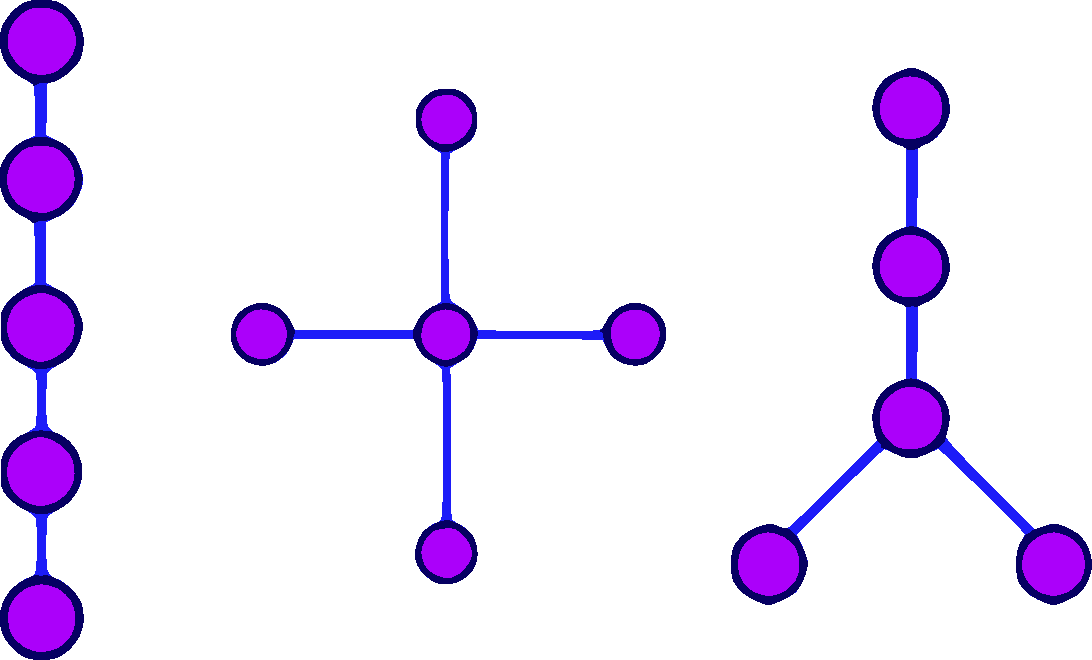
\includegraphics[width=0.4\textwidth]{3/img/arboles}
    \caption{Árboles correspondientes a cinco puntos.}
\label{isomeros_pentano}
\end{figure}

Donde un árbol es un tipo especial de grafo, distinto a los de los puentes de
K\"onigsberg, debido a que ahora no es necesario tener un camino, una ruta en
el caso de los puentes empieza y termina en él, en lo que se llama un ciclo.
Mientras que para un árbol no se tiene ningún ciclo.

Otras aplicaciones de la topología en la ciencia son:
\begin{itemize}
\item Efecto Hall Cuántico
\item Aislantes Topológicos
\item Estados Topológicos
\end{itemize}


\section{Generalidades Mecanocuánticas}

La mecánica cuántica es una de las piedras angulares de la física desde inicios
del siglo XX, la cuál ha sido empleada en el estudio de fenómenos micro-
nanoscópicos, para los cuales la mecánica clásica (newtoniana, lagrangiana o
hamiltoniana), no puede proporcionar predicciones congruentes con la evidencia
experimental. No obstante, muchas de las entidades de la mecánica analítica
jugaron un papel clave para el nacimiento de la mecánica cuántica. A pesar del
éxito de la mecánica cuántica en la resolución de muchos problemas, la
extrapolación de varias interpretaciones de la mecánica cuántica, en el mundo
macroscópico, ha llevado a varias discusiones entre las distintas ramas de la
física. Por ejemplo, aún no existe un acuerdo entre los postulados de la
mecánica cuántica y la relatividad general, siendo la ecuación de Dirac el
único puente entre la relatividad especial y la mecánica cuántica. La ecuación
de Dirac describe partículas elementales masivas de espín $\sfrac{1}{2}$ como
los electrones o los \textit{quarks}~\cite{Halzen1984}.

La teoría más exitosa de la física, hasta ahora, se fundamenta en la mecánica
cuántica, ésta se trata del Modelo Estándar de la Física de Partículas. Esta
teoría de campos describe tres de las cuatro interacciones fundamentales
(fuerza fuerte, fuerza débil y fuerza electromagnética)~\cite{Cheng1984}, y lo
hace de forma exitosa, detalla fenómenos como el momento magnético anómalo del
electrón con hasta diez cifras de exactitud, además predijo la existencia de
partículas antes de su descubrimiento experimental como es el caso de los
bosones W, Z, Higgs, y el gluón~\cite{Kinoshita2006}.  Sin embargo no es
posible explicar con dicha teoría: $i$) la masa del neutrino, $ii$) el momento
magnético anómalo del muón, $iii$) la materia obscura, $iv$) la constante
cosmológica, además de no integrar la gravedad.

Son necesarios entonces nuevos modelos, física más allá del modelo estándar.
La búsqueda de una teoría de la gravedad cuántica ha dado paso a numerosos
estudios teóricos, teniendo que agregar conceptos tales como: súper simetría,
acoplamiento fuerte, dimensiones extra o gravedad modificada, nada de esto
encontrado aún a través de experimentos u observaciones.  Dentro de las teorías
más famosas se encuentran la teoría de supercuerdas y la teoría cuántica de
bucles, ambas con aciertos, pero también con fallas que aún no han podido ser
resueltas.

La radiación emitida en el horizonte de eventos de un agujero negro fue el
primer acercamiento de constantes provenientes tanto de la cuántica como de la
gravitación, esta radiación fue descrita por Stephen
Hawking~\cite{HAWKING1974}, la cual relaciona el principio de indeterminación
de Heisenberg con las singularidades espacio-temporales; ésta radiación es
emitida debido a que tras la creación de un par partícula-antipartícula cerca
del horizonte de eventos de un agujero negro, una de las partículas queda
atrapada mientras la otra logra escapar del pozo gravitatorio. Debido a esta
radiación es posible dar dos implicaciones: $i$) los agujeros negros se están
evaporando y $ii$) a los agujeros negros se les puede asociar una temperatura
no nula, como se describe en la siguiente ecuación,
%
\begin{align}
T_{H} = \frac{\hbar c^{3}}{8\pi GM k_{B}}.
\end{align}

Como se mencionó, uno de los grandes problemas de la mecánica cuántica, resulta
de la extrapolación de los resultados del mundo microscópico al mundo
macroscópico. El mejor ejemplo es la superposición cuántica, este fenómeno es
extrapolado al mundo macroscópico con la tan socorrida paradoja del gato de
Schr\"odinger; dicha paradoja es inexistente, ya que las contribuciones
cuánticas se ven colapsadas al tratarse de objetos macroscópicos
%(un gato, el veneno y el detector),
y al no poderse aislar el sistema de él mismo, debido a que el gato emitirá
radiación de cuerpo negro de distinta manera si está vivo o muerto.
%la súper posición cuántica se verá colapsada.
Esta paradoja fue propuesta como un experimento mental (gedankenexperiment),
por el mismo Schr\"odinger en 1935 para ilustrar la superposición de estados
cuánticos y como la mecánica cuántica es contraintutiva. Ninguna interpretación
de la mecánica cuántica es realmente concluyente, en palabras de Richard
Feynman ``{\em I think I can safely say that nobody understands quantum
mechanics}''.

A pesar de lo anterior, la mecánica cuántica ha ayudado en varias ramas de la
ciencia, como es el caso de problemas donde la química y la física tienen una
frontera difusa, es aquí donde el la función de estado, $\psi$, es de gran
utilidad. El estudio de esta función permite obtener mucha información del
sistema de interés y, a pesar de no tener significado físico por sí sola, su
cuadrado puede ser interpretado como la amplitud de la probabilidad de
presencia de materia, en un intervalo de posición para la(s) partícula(s) de
estudio.

Una de las expresiones más importantes dentro de la mecánica cuántica es la
Ecuación de Schr\"odinger dependiente del tiempo, que para el caso de una
partícula, se escribe como:
%
\begin{align}
i\hbar \frac{\partial}{\partial t} \Psi (\mathbf{r}, t) = 
\left [ \frac{-\hbar^2}{2m}\nabla^2 + V(\mathbf{r},t) \right ] \Psi (\mathbf{r}, t),
\end{align}
%\begin{align}
%\hat{H}|\Psi (t)\rangle = i\hbar\frac{d}{dt}|\Psi (t)\rangle =
%\frac{\hat{\vec{p}}^{\ 2}}{2m}|\Psi (t)\rangle + V(\hat{\vec{r}}, t)|\Psi\rangle
%\end{align}
%
%i\hbar \frac{\partial}{\partial y}\Psi (\mathbf{r}, t) =
%\hat{H} (\mathbf{r}, t)\Psi(\mathbf{r}, t)

\noindent donde $\Psi (\mathbf{r}, t)$
es la función de estado
asociada al sistema.
%\noident

Debido a su simplicidad, la ecuación de Schr\"odinger dependiente del tiempo es
de gran utilidad, sin embargo, la resolución de problemas de eigenvalores que
resulta de la ecuación de Schr\"odinger independiente del tiempo es de mayor
utilidad para la química cuántica,
%
\begin{align}
\widehat{H}\Psi = E\Psi ,
\end{align}

\noindent donde $\widehat{H}$ es el operador Hamiltoniano, $\Psi$ es la
eigenfunción de dicho operador y es la función de estado del sistema, por
último $E$ es el eigenvalor que representa a la energía total del sistema.

Cabe resaltar que, con excepción del átomo y la molécula de hidrógeno, no hay
soluciones analíticas para la ecuación de Schr\"odinger en sistemas de interés
químico, por lo que se recurre a diversas aproximaciones y a sistemas
iterativos para una obtención de resultados útiles dentro de la química
cuántica.

\subsection{Método variacional}

Debido al interés por resolver un problema de eigenvalores como lo es la
ecuación de Schrödinger, la cual no cuenta con soluciones exactas para sistemas
con varios electrones, se requiere el uso de métodos aproximados, como lo es el
método variacional que permite conseguir soluciones aproximadas a problemas con
eigenvalores, $\widehat{O}\varphi = \omega\varphi$. Es común usar este método
para calcular la energía de sistemas atómicos y moleculares de $N$ electrones.

Sea $\widehat{A}$ un operador hermitiano y exista un conjunto infinito de
soluciones exactas a la ecuación de valores propios de modo que:
%
\begin{align}
  \widehat{A}|\phi_{\alpha} \rangle = \epsilon_{\alpha}|\phi_{\alpha} \rangle \qquad donde:\ 
  \epsilon_{0} \le \epsilon_{1} \le \ldots \le \epsilon_{\alpha}
  \le \ldots
\label{val_schr}
\end{align}

Si suponemos que el conjunto ${\epsilon_{\alpha}}$ es un conjunto de valores
discretos, las correspondientes eigenfunciones son ortonormales y se multiplica
por la izquierda por $\langle\phi_{\beta}|$ a la Ecuación \ref{val_schr}
obtenemos:
%
\begin{align}
\langle\phi_{\beta} |\widehat{A} | \phi_{\alpha}\rangle = \epsilon_{\alpha}\delta_{\alpha\beta}.
\end{align}

Debido a que las eigenfunciones de $\widehat{A}$ forman un conjunto completo,
cualquier función $\varphi$ es combinación lineal de las $\phi_{\alpha}$ si y
sólo si $\varphi$ satisface las condiciones de frontera del sistema
~\cite{szabo},
%
\begin{align}
  |\varphi\rangle = \sum_{a}|\phi_{\alpha}\rangle c_{\alpha} = 
  \sum_{a}|\phi_{\alpha}\rangle\langle\phi_{\alpha} |\varphi\rangle,
\end{align}
\noindent y
\begin{align}
  \langle\varphi| = \sum_{a}c^{\star}_{\alpha} \langle\phi_{\alpha}|= 
  \sum_{a} \langle\varphi | \phi_{\alpha} \rangle \langle\phi_{\alpha}.
\end{align}

El teorema variacional enuncia que si en un sistema con $i$) un Hamiltoniano
independiente del tiempo, $ii$) el eigenvalor correspondiente al estado basal
es $\varepsilon_{0}$ y $iii$) $\varphi$ es una función normalizada que
satisface las condiciones de frontera, entonces
%
\begin{align}
\langle \varphi |\widehat{H}| \varphi \rangle \ge \varepsilon_{0}.
\end{align}

La minimización de la energía electrónica partiendo de una función de estado es
la base del método variacional, tras la optimización de los parámetros a los
cuales está sujeta la función de estado, se obtiene dicha función del estado
basal. Este método es utilizado en el cálculo de variaciones, desarrollando
métodos generales para encontrar funciones que limitan los valores de las
cantidades dependientes de dichas funciones.

\subsection{Hartree-Fock}

Una de las primeras ideas para dar solución, de manera aproximada, al problema
mecanocuántico de la ecuación de Schr\"odinger para sistemas con muchos
electrones fue desarrollada, a la par y de manera independiente, por Douglas
Hartree y Vladimir Fock. La principal suposición en dicha aproximación es que
cada electrón interacciona con el resto de la misma manera en la que
interacciona con una densidad electrónica y no como con partículas
independientes, de modo que la ecuación ya no es una función de las $3(N-1)$
coordenadas espaciales de resto de electrones, sino de sólo la distancia $r$.
Esta idea es llamada aproximación de campo central, tomando un promedio
esférico que se expresa como:
%
\begin{align}
V_{1}(r_{1})=\frac{1}{4\pi}\int_{0}^{2\pi}\int_{0}^{\pi} V_{1}(\vec{r}_1)\sin\theta
\mathrm{d}\theta \mathrm{d}\varphi.
\end{align}

Para llevar a cabo la aproximación de un sistema polielectrónico se recurre al
uso de sistemas monoelectrónicos, es necesario tomar una aproximación orbital
(producto de Hartree), como se muestra en la Ecuación \ref{Aprox_Orb}, y para
garantizar la antisimetría ante el intercambio usamos el determinante de Slater
como se muestra en la Ecuación \ref{det_s}, que se suele denotar, por
simplicidad, como la Ecuación \ref{det_s_2}.
%
\begin{align}
  \Psi = \prod_{i=1}^{n} s_i (\vec{r_i}) ,
\label{Aprox_Orb}
\end{align}
\begin{align}
  |\Psi_0\rangle = \frac{1}{\sqrt{N!}}
  \begin{vmatrix}
    \phi_{1}(\mathbf{x}_1) & \phi_{2}(\mathbf{x}_1) & \cdots & \phi_{N}(\mathbf{x}_1) \\
    \phi_{1}(\mathbf{x}_2) & \phi_{2}(\mathbf{x}_2) & \cdots & \phi_{N}(\mathbf{x}_2) \\
    \vdots & \vdots & \ddots & \vdots \\
    \phi_{1}(\mathbf{x}_N) & \phi_{2}(\mathbf{x}_N) & \cdots & \phi_{N}(\mathbf{x}_N)
  \end{vmatrix} ,
\label{det_s}
\end{align}
%
\begin{align}
  |\Psi_0\rangle = |\phi_{1}\phi_{2} \cdots \phi_{N} \rangle ,
\label{det_s_2}
\end{align}

\noindent donde $\phi$ y $\mathbf{x}_n$ representa un espín-orbital y las
coordenadas espaciales y de espín de cada electrón respectivamente,
$\frac{1}{\sqrt{N!}}$ es la constante de normalización.

La energía del sistema en HF es expresada a través de la Ecuación
\ref{HF_energy}, y mediante el principio variacional es posible obtener una
mejor función de estado, debido a que es la que proporcione la menor energía,
pero esto depende de la elección de los espín-orbitales.
%
\begin{align}
  E_0 = \langle \Psi_0 | \widehat{H}_{el} | \Psi_0 \rangle .
\label{HF_energy}
\end{align}

El minimizar la Ecuación \ref{HF_energy} sumado a la restricción de
ortonormalidad de los espín-orbitales $\langle\phi_{i}|\phi_{j}\rangle =
\delta_{ij}$ dan paso a la ecuación HF,
\begin{align}
  \widehat{F}\phi_{i}(\mathbf{x}_i)=\varepsilon_{i}\phi_{i}(\mathbf{x}_i),
\end{align}

\noindent donde $\widehat{F}$ es el operador de Fock y $\varepsilon_i$ es la
energía del $i$-ésimo espín-orbital $\phi_i$. La repulsión electrónica dentro
del operador de Fock es tratada como un promedio, expresándose como:
%
\begin{align} %Operador HF
  \widehat{F} (i) = \widehat{h}(i) + \sum_{b=1}^{Ne} [\hat{J}_b (i) - \hat{K}_b (i)],
\end{align}

\noindent donde $\widehat{h}(i)$ es la suma de los operadores de energía
cinética y la atracción con los núcleos, los operadores $\hat{J}_b$ y
$\hat{K}_b$ son los operadores de Coulomb (electrostático) y de intercambio
(sin interpretación clásica debido a ser consecuencia de la antisimetría),
respectivamente, 
%
\begin{align}
  \widehat{h}(i) = -\frac{1}{2}\nabla^{2}_{i} -\sum_{A=1}\frac{Z_{A}}{r_{iA}}, \ \ 
  \hat{J}_b (1) = \langle\phi_{b}(2) h(12) \phi_{b}(2)\rangle , \ \ 
  \hat{K}_b (1) =\langle\phi_{b}(2) h(12) \phi_{a}(2)\rangle ,
\end{align}

\noindent los operadores $\hat{J}$ y $\hat{K}$ son parte del término
bielectrónico y suelen ser utilizados también como las integrales de Coulomb y
de intercambio, de la siguiente manera:
%
\begin{align}
  J_{ij} \equiv \int\frac{\phi_{i}^{\star}(i)\phi_{j}^{\star}(j)\phi_{i}(i)\phi_{j}(j)}{r_{ij}}
  d^{3}\tau_{i}d^{3}\tau_{j} =
  \int\frac{\rho_{i}(i)\rho_{j}(j)}{r_{ij}}d^{3}\tau_{i}d^{3}\tau_{j},
\end{align}
\begin{align}
  K_{ij} \equiv \int\frac{\phi_{i}^{\star}(i)\phi_{j}^{\star}(j)\phi_{i}(j)\phi_{j}(i)}{r_{ij}}
  d^{3}\tau_{i}d^{3}\tau_{j} ,
\end{align}
%
\noindent también expresados como:
\begin{align}
  \begin{split}
    J_{ab} & \equiv \langle\phi_{a}(1)\phi_{b}(2)h(12)\phi_{a}(1)\phi_{b}(2) \rangle \\
	         & = \langle\phi_{a}(1) \hat{J}_{b}(1) \phi_{a}(1) \rangle ,
  \end{split}
\end{align}

\begin{align}
  \begin{split}
    K_{ab} & \equiv \langle\phi_{a}(1)\phi_{b}(2)h(12)\phi_{a}(2)\phi_{b}(1) \rangle \\
	         & = \langle\phi_{a}(1) \hat{K}_{b}(1) \phi_{a}(1) \rangle .
  \end{split}
\end{align}

Con lo anterior es posible reescribir la Ecuación de Fock como se muestra en la
Ecuación \ref{HF_forall}, y ésta debe ser resuelta de manera autoconsistente,
es decir, la solución de las ecuaciones de Fock se lleva a cabo mediante un
proceso iterativo, por lo que es necesario iniciar a partir de un conjunto
inicial de espín-orbitales, con la que se construye el operador de Fock y
determinan las eigenfunciones de $\widehat{F}$, con éstas se vuelve a construir
nuevamente el operador de Fock hasta que las funciones con las que se construye
$\widehat{F}$ y sus eigenfunciones se aproximen tanto como uno lo desee.
%
\begin{align}
\left(\widehat{h}(i) + \sum_b [\hat{J}_b (i) - \hat{K}_b (i)]\right)\phi_a (i) =
\varepsilon_a \phi_a (i) \qquad \forall a \in (1,Ne) .
\label{HF_forall}
\end{align}

Esta aproximación es muy importante para sistemas químicos, además de
proporcionar funciones de estado y la energía del sistema, es un muy buen punto
de partida para diversos métodos aproximados posteriores a HF.

Las ecuaciones de Hartree-Fock no son lineales, además de ser ecuaciones
integro-di\-fe\-ren\-cia\-les por lo que resultan complicadas de resolver. Por
lo que se recurre a métodos como el propuesto por Roothaan en
1951~\cite{Roothaan1951} en el cual lo orbitales HF son combinaciones lineales
de un conjunto de funciones conocidas, funciones base~\cite{levine}. Esta
aproximación es conocida como el método de campo autoconsistente (SCF por sus
siglas en inglés), SCF se fundamenta en usar un conjunto de funciones base para
representar los espín-orbitales buscados, donde la base está normalizada, mas
no necesariamente es ortogonal.
%
\begin{align}
  \chi_{i} = \sum_{\nu} C_{\nu i}\phi_{\nu},
\end{align}

\noindent ${\phi_{\nu}}$ representa al conjunto base y $C_{\nu i}$
son los coeficientes de cada espín-orbital; en un conjunto completo de funciones se
obtiene la solución exacta de las ecuaciones.

\begin{wrapfigure}{l}{0.52\textwidth}
    \centering
    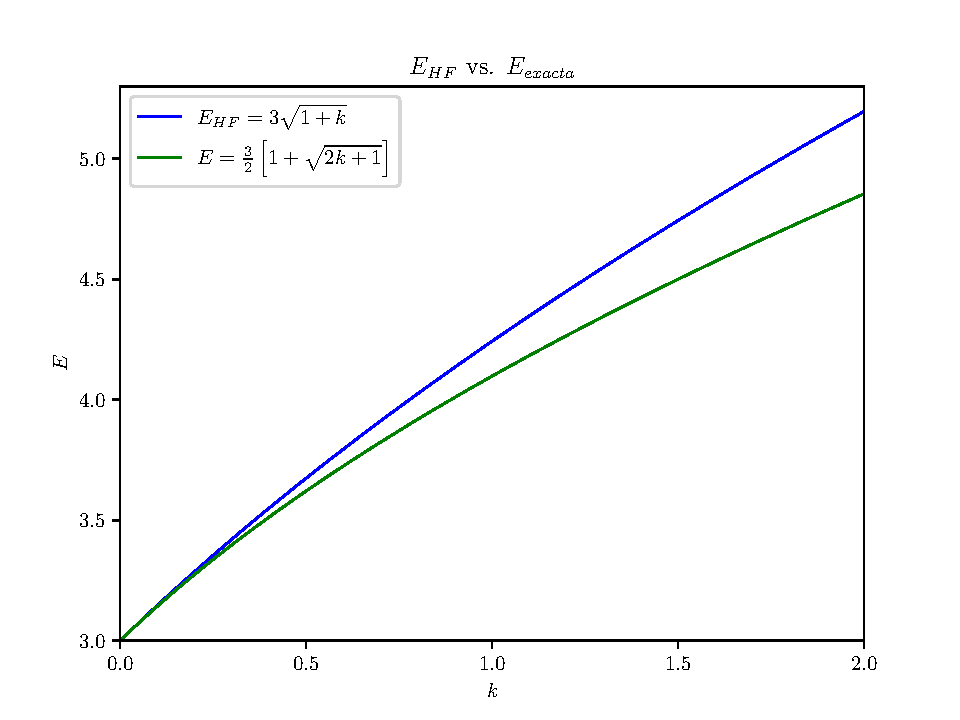
\includegraphics[width=0.55\textwidth]{3/img/HF_vs_excat}
    \caption{Gráfico presentado en \citenum{Moshinsky}.}
\label{HF_vs_excat}
\end{wrapfigure}
%
Pero, ?`qué tan buena es la aproximación HF?  Los principales problemas que se
tienen en la aproximación HF son $i$) no respeta el postulado de exclusión de
Pauli, $ii$) en la Aproximación de Campo Central (CFA) los armónicos esféricos
no tienen que ser funciones propias de la ecuación monoelectrónica, $iii$) no
existe una manera obvia de mejorar la aproximación orbital, y $iv$) no
considera efectos de correlación, que no necesariamente son despreciables en
todos los casos.

Para sistemas pequeños, a distancia corta y, más importante, sin mucha
correlación, es posible obtener buenos resultados tal como se muestra
en~\citenum{Moshinsky}, para la energía es posible tener el 95 \% del valor de
la energía exacta, pero sólo teniendo el 65 \% para el traslape. En la Figura
\ref{HF_vs_excat} es posible observar como la aproximación HF se aleja de la
solución exacta.

Por lo que usar HF para química cuántica puede ser un método barato en términos
computacionales y funcional para sistemas peque'nos, pero malo para abordar
otro tipo de problemas, como los que se pueden encontrar en física nuclear.

\section{Densidades}\label{densidades}

Uno de los términos importantes a definir, dentro de la fisicoquímica teórica,
es el de la densidad electrónica, $\rho (\vec{r})$, que, para un sistema de dos
electrones con coordenadas espín-espaciales $\vec{x}_{1}$ y $\vec{x}_2$, está
definida como: $|\Psi (\vec{x}_1 ,  \vec{x}_2)^2|$~\cite{RobertG1994}.  Para
calcular la probabilidad de hallar simultáneamente al electrón 1 en
$d\vec{x}_1$ y al 2 en $d\vec{x}_2$ se debe integrar la función denisdad sobre
$d\omega_1 d\vec{x}_2$, donde: $d\vec{x}_n =  d\vec{r}_n d\omega_n$
% y $d\vec{x}_2 = d\vec{r}_2 d\omega_2$,
\begin{align}
  P(\vec{r}_1)=\int |\Psi (\vec{x}_1 ,  \vec{x}_2)|^2 d\omega_1 d\vec{x}_2 ,
\end{align}

\noindent y, al ser los electrones partículas indistinguibles, llegamos a la
siguiente expresión:
\begin{align}
  \rho(\vec{r})=2\int |\Psi (\vec{x}_1 ,  \vec{x}_2)|^2 d\omega_1 d\vec{x}_2 ,
\end{align}

\noindent luego entonces, para un sistema con $N$ electrones la densidad
electrónica se puede generalizar de la siguiente manera:
\begin{align}
  \rho(\vec{r})=N\int |\Psi (\vec{x}_1 ,  \vec{x}_2,  \ldots , \vec{x}_N)|^2
  d\omega_1 d\vec{x}_2 \ldots d\vec{x}_N ,
\label{definition}
\end{align}

\noindent tal que:
\begin{align}
  \int\rho (\vec{r})d\vec{r} =N ,
\end{align}

\noindent en el caso de un determinante de Slater (Hartree-Fock), es posible
escribir a la densidad electrónica para una capa cerrada con orbitales
espaciales ${\psi_a}$ como:
\begin{align}
  \rho (\vec{r}) = 2 \sum_{a=1}^{N/2} |\psi_a (\vec{r})|^2 .
\end{align}

Para un sistema de $N$ partículas, es posible escribir un operador para la
densidad $\hat{\rho}$ y así obtener valores esperados a través de la función de
estado del sistema,
%
\begin{align}
  \hat{\rho} = \sum_i ^N \delta (\hat{r}_i - \vec{r}_0),
\end{align}

\noindent por lo que $\rho (\vec{r})$ al ser un valor esperado de un operador
de la mecánica cuántica, se puede escribir como:
%
\begin{align}
  \rho (\vec{r})= \int\Psi^{\star} (\vec{x}_1, \ldots , \vec{x}_N)
  \sum_i ^N \delta (\hat{r}_i - \vec{r}_0) \Psi (\vec{x}_1, \ldots , \vec{x}_N)
  d\vec{x}_1 \ldots d\vec{x}_N .
\end{align}

El valor de la densidad electrónica es muy importante, debido a que es un valor
que se puede obtener de manera experimental. Los experimentos de los que
podemos obtener información de $\rho (\vec{r})$ son la difracción de Rayos X o
la difracción de neutrones~\cite{Kasai2018, Coppens1971}. Por lo que cotejar
los valores teóricos con los experimentales dan una idea de que tan bien se
están tomando las consideraciones teóricas para los cálculos.
%
%\subsection{Densidad eletrónica, de espín y otras funciones de densidad}
% 
%La diferencia entre los componentes $\alpha$ y $\beta$ permite definir
%una densidad de espín, esencialmente como el exceso de densidad de los
%electrones ``up-spin'' comparados con los ``down-spin''. En a'nos recientes, con
%el desarrollo de mejores técnicas de resonancia magnética, esta cantidad ha
%cobrado más importancia. Para indicar el valor esperado, usamos la componente
%$z$ del momento angular del espín, por lo que podemos escribir:
%%
%\begin{align}
%\langle S_z \rangle = \int\limits_{\mathbf{x}'_1 = \mathbf{x}_1} S_{z} (1)\rho
%(\mathbf{x}_1, \mathbf{x}'_1) d\mathbf{x}_1
%\end{align}
%
%Ahora para el eigenestado de cualquier espín, $\rho$ puede ser expresado
%en términos de estos componentes, y la integración del espín, queda
%escrita como:
%%
%\begin{align}
%\langle S_z \rangle = \int\limits_{\mathbf{x}'_1 = \mathbf{x}_1} \frac{1}{2}
%\left[ P_{\alpha} (\mathbf{r}_{1} , \mathbf{r}'_{1}) - P_{\beta} (\mathbf{r}_{1} , \mathbf{r}'_{1})
%\right]
%d\mathbf{r}_1
%\end{align}
% 
%Para $\mathbf{x}'_1 = \mathbf{x}_1$, el integrando representa la contribución
%del valor esperado para un elemento de volumen $d\mathbf{r}$ en un espacio
%tridimensional ordinario. Definimos además:
%%
%\begin{align}
%Q_z (\mathbf{r}_1 , \mathbf{r}'_{1}) = \frac{1}{2}
%\left[ P_{\alpha} (\mathbf{r}_{1} , \mathbf{r}'_{1}) - P_{\beta} (\mathbf{r}_{1} , \mathbf{r}'_{1})
%\right]
%\end{align}
% 
%\noindent como la matriz de densidad de espín. Es de notar que en los elementos
%de la diagonal $\mathbf{r}'_1 = \mathbf{r}_{1}$, es simplemente la densidad
%del momento angular del espín en el eje $z$. Es claro ver que $Q_z$ se extrae
%de manera sencilla de $\rho$ aplicando el operador de espín $S_z$ antes de
%integrarse sobre el espín.
%%
%\begin{align}
%Q_z (\mathbf{r}_1) = \int S_z \rho (\mathbf{x}_1) ds_1
%\end{align}
%
%Dado que para un eigenestado de espín, es un valor esperado, la
%expresión correspondiente a ese valor esperado es:
%%
%\begin{align}
%\langle S_z \rangle = \int Q_z (\mathbf{r}_1) d\mathbf{r}_1 = M
%\label{spin_den}
%\end{align}
%
%En su forma más general, la función de densidad (o distribución) de la
%Ecuación \ref{definition}, de un electrón
%puede escribirse separando las partes espaciales y de espín, como se mostró
%al inicio de esta sección, sólo que ahora se mostrará con otra notación:%~\cite{Magnasco2009}:
%\begin{align}
% \begin{split}
%\rho_1 (\mathbf{r}_1 s_1 ; \mathbf{r}_1 s_1) & =
%\rho_1^{\alpha\alpha} (\mathbf{r}_1;\mathbf{r}_1)\alpha (s_1)\alpha^{\star} (s_1) +
%\rho_1^{\beta\beta} (\mathbf{r}_1;\mathbf{r}_1)\beta (s_1)\beta^{\star} (s_1)  \\
%&+ \rho_1 ^{\alpha\beta} (\mathbf{r}_1;\mathbf{r}_1)\alpha (s_1) \beta^{\star} (s_1) +
%\rho_1 ^{\beta\alpha} (\mathbf{r}_1;\mathbf{r}_1)\beta (s_1) \alpha^{\star} (s_1)
% \end{split}
%\end{align}
%
%\noindent donde las $\rho$'s son ahora solo funciones espaciales. Al integrar sobre
%el espín, los dos últimos términos desaparecen, debido a la ortogonalidad de las
%funciones de espín, y nos quedan las cantidades sin espín
%%
%\begin{align}
%\rho_1 ^{\alpha\alpha}(\mathbf{r}_1 ; \mathbf{r}_1 ) =
%\rho_1 ^{\alpha}(\mathbf{r}_1 ; \mathbf{r}_1 ),
%\	\rho_1 ^{\beta\beta}(\mathbf{r}_1;\mathbf{r}_1) =
%\rho_1 ^{\beta}(\mathbf{r}_1;\mathbf{r}_1)
%\end{align}
%
%\noindent con el significado físico de: $
%\rho_1 ^{\alpha}(\mathbf{r}_1 ; \mathbf{r}_1 )d\mathbf{r}_1 =$ probabilidad de encontrar
%en $d\mathbf{r}_1$ un electrón con espín $\alpha$, y
%$\rho_1 ^{\beta}(\mathbf{r}_1 ; \mathbf{r}_1 )d\mathbf{r}_1 =$ probabilidad de encontrar
%en $d\mathbf{r}_1$ un electrón con espín $\beta$
%
%Usando la definción de la ecuación \ref{definition}, omitiendo el sufijo 1 (obviable por el
%momento), la integración sobre $d\mathbf{x}_2$, da como resultado la distribución de
%un electrón:
%\begin{align}
%\rho_1 (\mathbf{x} ; \mathbf{x})=\phi (\mathbf{r}) \phi^{\star} (\mathbf{r})
%[\alpha (s) \alpha^{\star} (s) + \beta (s) \beta^{\star} (s)]
%\end{align}
%
%\noindent de modo que:
%\begin{align}
%\rho_1^\alpha (\mathbf{r} ; \mathbf{r}) = \rho_1^\beta (\mathbf{r} ; \mathbf{r}) =
%\phi (\mathbf{r}) \phi^{\star} (\mathbf{r}) = R (\mathbf{r} ; \mathbf{r})
%\end{align}
%
%Los coeficientes de $\alpha \alpha^{\star}$ y $\beta\beta^{\star}$ son iguales para los orbitales
%moleculares doblemente ocupados y generalmente se denotan por R.
%Luego obtenemos las densidades de electrones y espines de nuestro enlace
%orbital~\cite{Magnasco2009}.
%\begin{align}
%P(\mathbf{r} ; \mathbf{r})= \rho_1^\alpha (\mathbf{r} ; \mathbf{r}) +
%\rho_1^\beta (\mathbf{r} ; \mathbf{r}) = 2R(\mathbf{r} ; \mathbf{r}) =
%2\phi (\mathbf{r})\phi^{\star} (\mathbf{r})
%\end{align}
%
%Retomando \ref{definition}, el término entero para la energía es posible
%escribir la siguiente expresión, la cual será de mayor  utilidad para la siguiente
%discusión:
%%
%\begin{align}
% \begin{split}
%E  & = -\frac{1}{2}\int\nabla^{2} P(\mathbf{r}_1) d\mathbf{r}_1 + \int VP(\mathbf{r}_1)d\mathbf{r}_1
%-\frac{1}{2}\int g\Pi (\mathbf{r}_{1}, \mathbf{r}_{2}) d\mathbf{r}_{1} d\mathbf{r}_2 \\
%& = T + V_{en} + V_{ee} \\
%\label{defE}
% \end{split}
%\end{align}
%
%La densidad de carga $P(\mathbf{r})$ y la densidad de espín $Q_z (\mathbf{r})$
%son ejemplos de propiedades
%puntuales o subobservables. Sus valores se infieren (nunca directamente medidos)
%por medio de una
%integral como $V_{en}$ en \ref{defE} que define un valor esperado. Por lo tanto,
%$VP(\mathbf{r})$ en \ref{defE} puede
%interpretarse como una densidad de energía potencial, ya que es la contribución
%por unidad de volumen a $V_{en}$ evaluada en el punto $\mathbf{r}$; y de forma
%similar, \ref{spin_den} $Q_z (\mathbf{r})$ se
%interpreta como una densidad de momento angular de espín.  Podría haberse
%esperado que otras densidades de propiedad pudieran definirse exactamente de la
%misma manera. Por lo tanto, refiriéndonos nuevamente a la Ecuación \ref{defE},
%%
%\begin{align}
%T(\mathbf{r})= \left[ \frac{p^2}{2m} P(\mathbf{r}; \mathbf{r'}) \right] _{\mathbf{r}'=\mathbf{r}} \
%(\hat{p}^2=\hat{p_x}^2 + \hat{p_y}^2 + \hat{p_z}^2)
%\end{align}
%
%\noindent parecería ser una densidad de energía cinética, debido a que
%$T(r\mathbf{r})d\mathbf{r}$ es la contirbución a 
%$\langle T\rangle$ asociada con el elemento de volumen $d\mathbf{r}$ en
%la posición. Sin embargo,
%existen dificultades con tales definiciones en la medida en que las
%contribuciones puntuales a observables reales no son necesariamente reales.
%Esto se debe a que en realidad, los valores de expectativa de los operadores
%Hermitianos (e incluso la definición del carácter Hermitaino), depende de la
%integración en todo el dominio de las variables. Las definiciones alternativas
%de una densidad de propiedad que dan el mismo valor de esperado cuando se
%integran en todo el espacio pueden dar valores locales muy diferentes (y no
%reales)~\cite{mcweeny}.  La definición aceptable simple de una densidad
%de energía cinética se expresa como:
%%
%\begin{align}
%T(\mathbf{r})= \left[ \frac{\hat{\mathbf{p}}\cdot \hat{\mathbf{p}}^{\dagger}}{2m} P(\mathbf{r}; \mathbf{r'}) \right] _{\mathbf{r}'=\mathbf{r}}
%\end{align}
%
%\noindent donde se entiende que el operador adjunto sólo trabaja en
%la variable primada.
%
%Esto proporciona el valor de expectativa habitual $\langle T\rangle$ cuando
%se integra en todo
%el espacio, pero tiene la ventaja conceptual de ser tanto real como positivo en
%todos los puntos~\cite{helgaker}.

Ahora bien, también es posible expresar una función de densidad para un par de
electrones, o densidad de pares, tal que:
%
\begin{align}
  \rho_2(\vec{r_1},\vec{r_2})=N(N-1)\int |\Psi (\vec{x}_1 ,  \vec{x}_2,  \ldots , \vec{x}_N)|^2
  d\omega_1 d\omega_2  d\vec{x}_3 \ldots d\vec{x}_N ,
\label{d_pares}
\end{align}

\noindent donde la densidad de pares,
$\rho_2(\vec{r}_1,\vec{r}_2)N^{-1}(N-1)^{-1}$, determina la probabilidad por
volumen de encontrar simultáneamente a dos electrones en las posiciones
centradas en $\vec{r_1}$ y $\vec{r_2}$, y comúnmente se expresa como una suma
que involucra términos de pares independientes y correlacionados,
$\rho_2(\vec{r}_1, \vec{r}_2) = \rho(\vec{r}_1)\rho(\vec{r}_2) +
\rho_2^{xc}(\vec{r}_2, \vec{r}_1)$.

La importancia de estas dos densidades, la densidad electrónica y la densidad
de pares (Ecuaciones \ref{definition} y \ref{d_pares}, respectivamente), viene
de que partiendo de éstas, de la aproximación Born-Oppenheimer y de la matriz
reducida de primer orden (Ecuación \ref{m_r_1}) es posible determinar la
energía no relativista de un sistema molecular, en ausencia de campos externos,
%
\begin{align}
  E=&-\frac{1}{2}\int\nabla^{2}\rho_{1}(\vec{r}_1, \vec{r}^{\,\prime}_1) \biggr |_{\vec{r}^{\,\prime}_1 \rightarrow \vec{r}_1} d\vec{r}_1
      -\sum_{A}\int\frac{Z_A \rho_1 (\vec{r}_1)}{r_{1A}}d\vec{r}_1
      +\sum_{A\neq B}\frac{Z_A Z_{B}}{r_{AB}} \nonumber \\
      \phantom{=}&+\frac{1}{2}\int\int\frac{\rho (\vec{r}_1) \rho (\vec{r}_2)}{r_{12}} d\vec{r}_1 d\vec{r}_2
      -\frac{1}{2}\int\int\frac{\rho_2^{xc}(\vec{r}_1, \vec{r}_2)}{r_{12}} d\vec{r}_1 d\vec{r}_2 \nonumber \\
   =&\ T + V_{ne} + V_{nn} + V_{ee} + V_{xc}.
\label{E_b-o}
\end{align}

En la práctica, la Ecuación \ref{E_b-o} para un método de estructura
electrónica particular requiere expresar a las distribuciones de densidad en
función de la base orbital molecular, $\phi_i$,
%
\begin{align}
  \rho_1 (\vec{r}) = \sum_{ij} D_{ij}\phi_{i}(\vec{r})\phi_{j}(\vec{r}),
\end{align}
\begin{align}
  \rho_2 (\vec{r}_1, \vec{r}_2) = \sum_{ijkl}d_{ijkl}\phi_{i}(\vec{r}_1) \phi_{j}(\vec{r}_1)
  \phi_{k}(\vec{r}_2)\phi_{l}(\vec{r}_2),
\end{align}

\noindent donde $D_{ij}$ y $d_{ijkl}$ son los elementos de matriz de primer y segundo orden.

\subsection{Matrices de la densidad}

Sabemos que el valor esperado de cualquier operado se pude obtener como:
%
\begin{align}
	\begin{split}
    \langle \widehat{Q} \rangle & = \int\Psi^{\star}(x_{1},x_{2},\ldots,x_{n}) \widehat{Q} \Psi(x_{1},x_{2},\ldots,x_{n}) dx_{1}\ldots dx_{n} \\ 
	                              & = \int\widehat{Q}\Psi(x_{1},x_{2},\ldots,x_{n}) \Psi^{\star}(x^{\prime}_{1},x^{\prime}_{2},\ldots,x^{\prime}_{n}) dx_{1}\ldots dx_{n} ,
	\end{split}
\end{align}

\noindent haciendo hincapié de que el operado no actúa en la variables primadas.

Si tenemos un operador que involucra $m$ variables, con $m\le n$, podemos escribir:
%
\small
\begin{align}
	\begin{split}
    \langle \widehat{Q} \rangle & = \int\widehat{Q}\Psi(x_{1},\ldots , x_{m}, x_{m+1}, \ldots , x_{n})
    \Psi^{\star}(x_{1},\ldots , x_{m}, x_{m+1}, \ldots , x_{n}) dx_{1}\ldots dx_{n} \\
	& =\int dx_{1}\ldots dx_{m} \widehat{Q}\int\Psi(x_{1},\ldots , x_{m}, x_{m+1}, \ldots , x_{n})
	  \Psi^{\star}(x_{1},\ldots , x_{m}, x_{m+1}, \ldots , x_{n}) dx_{m+1}\ldots dx_{n}\\
	& =\int dx_{1}\ldots dx_{m} \widehat{Q} (x_{1}, \ldots , x_{m}) F_{m}
	  (x_{1}, \ldots , x_{m}; x^{\prime}_{1}, \ldots , x^{\prime}_{m}),
	\end{split}
\end{align}
\normalsize

\noindent con:
%
\footnotesize
\begin{align}
  F_{m}(x_{1}, \ldots , x_{m}; x^{\prime}_{1}, \ldots , x^{\prime}_{m}) =
  \int dx_{m+1}\ldots dx_{n} \Psi(x_{1},\ldots , x_{m}, x_{m+1}, \ldots , x_{n})
  \Psi^{\star}(x^{\prime}_{1},\ldots , x^{\prime}_{m}, x^{\prime}_{m+1}, \ldots , x^{\prime}_{n}).
\end{align}
\normalsize

Con esta función $F$ relacionada con la matriz de densidad de orden $m$, la cual se define como:
%
\begin{align}
  \Gamma_{m}(x_{1}, \ldots , x_{m}; x^{\prime}_{1}, \ldots , x^{\prime}_{m}) = {n \choose m}\int dx_{m+1}
  dx_{n} \Psi^{\star}(x^{\prime}_{1},\ldots , x^{\prime}_{m}, x^{\prime}_{m+1}, \ldots , x^{\prime}_{n}) \Psi(x_{1},\ldots ,x_{n}),
\end{align}

\noindent donde ${n \choose m}$ son las combinaciones de $n$ elementos tomando $m$ en $m$,
%
\small
\begin{align}
  {n \choose m} = \frac{n!}{m! (n-m)!}\, .
\end{align}
\normalsize

Existe una jerarquía entre las matrices de densidad según su orden,
\small
\begin{align}
  \begin{split}
    \Gamma_{m}(x_{1}, \ldots , x_{m}; x^{\prime}_{1}, \ldots , x^{\prime}_{m}) & = \frac{{n \choose m}}{{n \choose {m+1}}}
    \int dx_{m+1}\Gamma_{m+1}(1, \ldots , m, m+1;1^{\prime}, \ldots , m^{\prime}, (m+1)^{\prime}) \\
	    & = \frac{m+1}{n-m} \int dx_{m+1}\Gamma_{m+1}(1, \ldots , m, m+1;1^{\prime}, \ldots , m^{\prime}, (m+1)^{\prime}).
  \end{split}
\end{align}
\normalsize

Debido a que en química cuántica los operadores son mono- o bielectrónicos, las
matrices de densidad que resultan de interés son de primer y segundo orden.
Existiendo varios criterios de normalización, por ejemplo: $\frac{n(n-1)}{2}$ o
$n(n-1)$, expuestos L\"owdin y McWeeny
respectivamente~\cite{Lwdin1955,mcweeny},
%
\begin{align}
  \Gamma_{1} (x_1;x_1^{\prime}) = n\int\Psi^{\star}(1^{\prime}, 2^{\prime}, \ldots ,n^{\prime})\Psi(1, 2, \ldots , n) dx_{2} \ldots dx_{n},
  \label{m_primer_orden}
\end{align}
\begin{align}
  \Gamma_{2} (x_{1}, x_{2};x^{\prime}_{1},x^{\prime}_{2}) = \frac{n(n-1)}{2} \int\Psi^{\star}(1^{\prime}, 2^{\prime}, \ldots ,n^{\prime})
  \Psi(1, 2, \ldots , n) dx_{3} \ldots dx_{n}.
\end{align}

Para diversas aplicaciones resulta conveniente trabajar con la matriz de
densidad de primer orden, también llamada de Fock-Dirac, Ecuación
\ref{m_primer_orden}, que al integrar con respecto a la coordenada de espín se
obtiene la matriz de densidad reducida de primer orden,
%
\begin{align}
  \rho_{1}(r_{1},r^{\prime}_{1}) = \int\Gamma_{1} (x_{1};x_{1}^{\prime}),
  \label{m_r_1}
\end{align}

\noindent donde a diferencia de las funciones de densidad, los elementos de las
matrices de la densidad no tiene significado físico, exceptuando a la diagonal,
que para el caso de la matriz reducida de primer orden coincide con la densidad
electrónica.

En importante resaltar que la suma de los elementos de la matriz de densidad de
primer orden, que es una integral por el carácter continuo de los índices de la
matriz, nos da como resultado el número total de electrones del sistema.

Muchas de las propiedades de los sistemas polielectrónicos, y en particular la
energía, pueden expresarse como una función de la matriz de densidad de primer
orden y de la densidad bielectrónica.


\section{Teoría de los Funcionales de la Densidad}

La teoría de los funcionales de la densidad es una de la teorías más
importantes usadas en el área de la fisicoquímica teórica. Cabe resaltar que es
un método variacional donde el funcional de la energía electrónica es
minimizado con respecto a la densidad electrónica.  Este es un paso importante,
ya que pasamos de depender de la función de estado, a depender de la densidad
electrónica, por lo que tenemos beneficios computacionales en la resolución de
sistemas grandes.

La densidad electrónica es una magnitud escalar más fácil de calcular debido a
su dependencia de sólo las tres variables espaciales, al contrario de la
función de estado que depende de 3$N$ variables. Exceptuando los casos más
sencillos, se tiene el inconveniente de no contar de manera exacta con el
funcional relacionado a la energía del sistema.

Esta manera de entender a la mecánica cuántica es un claro ejemplo de la
interpretación de Copenhague, y si bien originalmente esta teoría no
contemplaba la dependencia en el tiempo, posteriormente fue empezada a ocuparse
dentro del margen de la mecánica cuántica relativista, siendo denotado
mayormente como TDDFT (Time-dependent Density Functional Theory).

En 1984 se publica una generalización de los teoremas de Hohenberg y Kohn por
parte de Runge y Gross para el caso dependiente del tiempo y éste establece que
existe una relación de uno a uno entre la densidad dependiente del tiempo $\rho
(\vec{r}, t)$ y el potencial externo de un cuerpo $v_{ext} (\vec{r}, t)$ para
un estado inicial~\cite{Runge1984}.
%La función de estado de muchos cuerpos que depende de 3$N$ variables es
%equivalente a la densidad que depende sólo de las tres variables espaciales, y
%que todas las propiedades de un sistema pueden determinarse a través de
%conocer a esta densidad.
A diferencia de DFT, no existe un principio de minimización general en la
mecánica cuántica dependiente del tiempo, por lo que su demostración es más
complicada. 

%Una de las propiedades más usadas de TDDFT es el régimen de respuesta lineal,
%que puede ser utilizado si una perturbación externa es pequeña en el sentido
%de que no destruye completamente la estructura del estado fundamental del
%sistema. En este caso,  se pude analizar la respuesta lineal del sistema,
%dando una gran ventaja ya que, a primer orden, la variación del sistema
%dependerá solamente de la función de estado fundamental para la que se pude
%usar las propiedades de DFT.
%
%La aplicación más popular de TDDFT es el cálculo de las energías de estados
%excitados de sistemas aislados y de sólidos. Dichos cálculos se basan en el
%hecho de que la función de respuesta lineal, es decir, cómo cambia la densidad
%de electrones cuando cambia el potencial externo, tiene polos en las energías
%de excitación exactas de un sistema. Dichos cálculos requieren, además del
%potencial de intercambio-correlación, el núcleo de correlación de intercambio,
%la derivada funcional del potencial de correlación de intercambio con respecto
%a la densidad.
%
El principal inconveniente de DFT es que si bien en principio es una teoría
exacta, sólo se puede aplicar de forma aproximada, lo que hace que los
resultados sean menos precisos que en otros métodos. Asimismo, no se trata
correctamente la interacción de intercambio, por lo que la energía
intercambio-correlación pude ser distinta dependiendo de como se aproxime el
cálculo. Por estas razones es común que se tenga una cierta división conforme
al uso de DFT, con defensores debido a que sus resultados son bastante buenos
para su coste computacional y que es una buena forma de abordar ciertos
sistemas con gran complejidad, mientras que los detractores a esta teoría
abordan el tema de que se trata más de un método semiempírico y que sus
resultados no son tan fiables como las de un tratamiento \textit{ab initio}
clásico.

Históricamente, los primeros acercamientos que se empezaron a tener sobre la
utilización de la densidad electrónica para obtener información sobre los
sistemas de estudio empezó en 1927 con los trabajos de Llewellyn Hilleth Thomas
y Enrico Fermi, donde la idea principal es tomar a la energía cinética en
términos de contribuciones núcleo-electrón y electrón-electrón, donde éstos
sean tratados como fenómenos puramente clásicos, en un gas uniforme de
electrones. Sea un sistema ficticio con una densidad electrónica constante:
\begin{align}
  {T}_{\mathrm{TF}}[\rho(\vec{r})]=\displaystyle\frac{3}{10}(3\pi^2)^{(2/3)}\int
  \rho^{(5/3)}(\vec{r})d\vec{r},
\end{align}

\noindent que al ser combinado con las interacciones en términos clásicos de
núcleo-electrón, electrón-electrón se obtiene la expresión de la energía de un
átomo de Thomas-Fermi, ésta aproximación es bastante útil para casos donde los
electrones no se encuentran muy amarrados al núcleo, como es el caso de los
metales alcalinos y medianamente los alcalinoterreos:
%
\begin{align}
  {E}_{\mathrm{TF}}[\rho(\vec{r})]=\displaystyle\frac{3}{10}(3\pi^2)^{(2/3)}\int
  \rho^{(5/3)}(\vec{r})d\vec{r}-Z\int\displaystyle\frac{\rho(\vec{r})}{r}d\vec{r} +
  \displaystyle\frac{1}{2}\int\int\displaystyle\frac{\rho(\vec{r_1})\rho(\vec{r_2})}{r_{12}}
  d\vec{r_1}d\vec{r_2}.
\end{align}

Este modo de abordar los problemas mecanocuánticos a través de la densidad
cobró más importancia con el uso de los Teoremas de Hohenberg-Kohn presentados
en 1964~\cite{Hohenberg1964}, donde se expone que la energía es un funcional de
la densidad y que además la densidad del sistema minimiza este funcional. Otro
gran paso que dio esta teoría fue un año después cuando Kohn y Sham demostraron
que a partir de la DFT es posible escribir una ecuación para orbitales de una
partícula, de los cuales se pude obtener la densidad~\cite{Kohn1965}. En la
actualidad es un método ampliamente utilizado, aunque en sus inicios era más
socorrido en física del estado sólido al considerarse como un método no muy
preciso para la química.

\subsection{Teoremas de Hohenberg-Kohn}
\subsubsection{Teorema 1}

La energía y, por lo tanto las demás propiedades del sistema, están
unívocamente determinados por la densidad electrónica; si dos sistemas de $N$
partículas se encuentran en potenciales externos $v_{1} (\vec{r})$ y $v_{2}
(\vec{r})$, con la misma densidad electrónica en el estado basal
$\rho(\vec{r})$, la diferencia entre $v_{1} (\vec{r})$ y $v_{2} (\vec{r})$ es
necesariamente una constante. Por lo que no hay más de dos potenciales para
describir el mismo estado basal.

Corolario: el potencial y todas las propiedades del sistemas están determinadas
de manera única a través de la densidad del estado fundamental, incluida la
función de estado para muchos cuerpos. De forma particular el funcional de HK,
definido como $F[\rho]=T[\rho]+U[\rho]$ es un funcional universal de la
densidad, por lo que no depende de forma explícita del potencial externo.

El valor del estado fundamental de cualquier observable es una función única de
la densidad electrónica exacta del estado fundamental.
\begin{align}
  \langle \psi |\widehat{A}|\psi \rangle = A[\rho_0 (r)].
\end{align}

\subsubsection{Teorema 2}

El funcional con el que se obtiene la energía del estado fundamental del
sistema proporciona la energía más baja, si y sólo si, la densidad de entrada
es la verdadera densidad del estado fundamental, es decir, la energía obtenida
del Hamiltoniano alcanza su mínimo absoluto cuando la densidad electrónica es
la del estado fundamental.

Para cual sea potencial $v_{ext}(\vec{r})$, y natural $N$ la función de densidad
$F[\rho]$ existe como:
%
\begin{align}
  E_{v, N} [\rho] = F[\rho] + \int v_{ext}(\vec{r})\rho(\vec{r}) d^{3}r ,
\end{align}

\noindent y se obtiene el valor mínimo de la densidad del estado fundamental
para $N$ electrones en el potencial $v_{ext}(\vec{r})$. El valor mínimo de
$E_{v, N} [\rho]$ es entonces la energía del estado fundamental de este
sistema.

El segundo teorema establece al valor exacto de la energía como el mínimo valor
del funcional, es decir, tenemos una cota inferior para el cálculo,
%
\begin{align}
  E_{0}\leq E[\rho]=T[\rho] + V_{Ne}[\rho]+V_{ee}[\rho].
\end{align}

\subsection{Aproximación Kohn-Sham}

Kohn-Sham propone una nueva aproximación para resolver el problema de muchos
electrones basándose en los teoremas de HK, el total de la energía del
funcional en un potencial externo $v_{ext}(\vec{r})$ puede ser descrito como:
\begin{align}
  E[\rho(\vec{r})] = T[\rho(\vec{r})] + \int v_{ext}(\vec{r})\rho(\vec{r})d^{3}r +
  V_{ee}[\rho(\vec{r})] , 
  \label{KS1}
\end{align}
\noindent con:
\begin{align}
  V_{ee}[\rho(\vec{r})] = \frac12 \int\int \frac{\rho(\vec{r})\rho(\acute{r})}{|\vec{r}-\acute{r}|}d^{3}r
  d^{3}\acute{r} + {E}_{xc}[\rho(\vec{r})] .
\end{align}

Donde el primer término de la Ecuación \ref{KS1} es la energía cinética
$T[\rho(\vec{r})]$, el segundo término es el potencial externo dado por el
arreglo de los núcleos y el último término es la contribución tanto clásica
como no clásica (intercambio-correlación detrás de la teoría de campo medio de
la interacción electrón-electrón). Para resolver las ecuaciones de Kohn-Sham es
necesario asumir un sistema de referencia con partículas no interactuantes, y
con la densidad del estado fundamental igual que la del sistema interactuante.
La ecuación para referirse al sistema puede escribirse de la siguiente manera:
\begin{align}
  E_{eff}|\psi_{i}\rangle = \left [-\sum_{i}\frac12\nabla^{2}_{i} + v_{eff}[\rho(\vec{r})]\right ]|
  \psi_{i} \rangle = \epsilon_{i}|\psi_{i}\rangle ,
\end{align}

\noindent con lo anterior podemos describir la energía cinética del sistema de
la siguiente manera:
\begin{align}
  T_{eff}[\rho(\vec{r})] = \sum_{i}\epsilon_{i} - V_{eff}[\rho(\vec{r})].
%T_{eff}[\rho(\vec{r})] = \sum_{i}n_{i}\epsilon_{i} - V_{eff}[\rho(\vec{r})].
\end{align}

La nueva pseudoenergía cinética forma el funcional de la energía de
intercambio-correlación $E_{xc}[\rho(\vec{r})]$ que se expresa como:
\begin{align}
  E_{xc}[\rho(\vec{r})] = T[\rho(\vec{r})] - T_{eff}[\rho(\vec{r})] +
  V_{ee}[\rho(\vec{r})] - J[\rho(\vec{r})] .
\end{align}

Usando el nuevo funcional de intercambio-correlación en la energía total del
sistema, derivando la nueva energía total para el sistema no interactuante, y
el potencial efectivo con respecto a $\rho(\vec{r})$ (que por conservación de
la densidad, $\int\rho(\vec{r})=N$, donde $N$ es el número total de
electrones), tenemos una expresión para resolver la ecuación de Schr\"odinger
de un electrón que se está moviendo en un potencial $v_{eff}$:
\begin{align}
  \left[-\frac12\nabla^2 + v_{eff}[\rho(\vec{r})]\right]\psi_{i}(\vec{r})=\epsilon_{i}\psi_{i}(\vec{r}).
\end{align}

Finalmente podemos obtener la energía del sistema interactuante:
\begin{align}
  E[\rho] = \sum_i\epsilon_i -\frac12\int\int\frac{\rho(\vec{r})\rho(\acute{r})}
  {|\vec{r}-\acute{r}|}d^3r d^3\acute{r}+ E_{xc}[\rho(\vec{r})] -
  \int\frac{\delta E_{xc}[\rho(\vec{r})]}{\delta\rho(\vec{r})}\rho(\vec{r})d^3r .
\end{align}

\subsection{Funcionales}

El término funcional es usado generalmente con tres diferentes significados, los cuales
se enuncian a continuación~\cite{1990}:
%
\begin{itemize}
\item En álgebra lineal, refiere a un mapeo lineal desde un espacio vectorial
$V$ en su campo escalar, es decir, se refiere a un elemento del espacio dual
$V^{*}$.
\item En análisis matemático, de manera más general e histórica, se refiere a
un mapeo desde un espacio $X$ a los números reales, o a veces a los números
complejos, con el propósito de establecer una estructura similar al cálculo en
$X$. Dependiendo del autor, tales mapeos se puede o no suponer que es lineal o
que se define en todo el espacio.
\item En computación, es sinónimo de funciones de orden superior, es decir,
funciones que toman funciones como argumentos o las devuelven.
\end{itemize}

Para la física y química teórica el uso de funcionales resulta de bastante
utilidad, tomando los significados anteriores se puede decir que ahora no se
depende de un escalar, vector, matriz o tensor de cualquier orden, sino de una
función entera y que su resultado sigue siendo un valor, a groso modo
\textit{una función de funciones}. Esto resulta ser bastante útil al poder
extrapolar varios conceptos ya conocidos de las matemáticas con esta nueva
herramienta; como la de definir una derivada funcional, útil para la mecánica
lagrangiana, o la de integrales funcionales que son la idea central para la
integración de camino expuesta por Richard Feynman.

Existen varios tipos de funcionales intercambio-correlación dentro de DFT y es
posible clasificar éstas a través del tipo de aproximaciones que se realizan.
%
\begin{itemize}

\item \textbf{Aproximación de la Densidad Local}, la densidad se modela como la de un gas
electrónico localmente homogéneo con densidad electrónica $\rho$.

$E_{xc}^{LDA} [\rho] = \int \rho (r) v_{xc}(\rho (r)) dr$

Ejemplos de funcionales de intercambio: Método de X$_{\alpha}$~\cite{Slater74},
Slater (LSDA)~\cite{Slater74}.

Ejemplos de funcionales de correlación: VWN~\cite{Vosko1980},
PL~\cite{Perdew1981}.
\item \textbf{Aproximación del Gradiente de la Densidad}, además de la densidad se incluye
el gradiente.

$E_{xc}^{GGA} [\rho] = \int \rho (r) v_{xc}(\rho (r), \nabla\rho (r)) dr$

Se suelen construir como una corrección que se añade al funcional LDA.

Ejemplos de funcionales de intercambio:
B (Becke)~\cite{Becke1988}, mPW~\cite{Adamo1998}.

Ejemplos de funcionales de correlación:
P86~\cite{Perdew1986}, LYP~\cite{Lee1988}.
\item \textbf{Meta-GGA}, incluyen también el laplaciano de la densidad $\nabla^{2}\rho (r)$; en
la práctica utilizan la densidad de energía cinética.

$\tau (r) = \displaystyle\sum_{i}^{N} \displaystyle\frac12 |\nabla\psi_i (r)|^{2}$

$E_{xc}^{MGGA} [\rho] =\int\rho (r) v_{xc}(\rho (r), \nabla\rho (r), \tau (r)) dr$

Ejemplos: KCIS~\cite{1999}, VSXC~\cite{VanVoorhis1998}.
\item \textbf{Funcionales Híbridos}, incluyen una parte de la energía de intercambio exacta de HF,
que se calcula a partir de los orbitales KS.

$E_{x}^{HF} [\theta_{i}] = -\displaystyle\sum_{i=1}^{N/2}\displaystyle\sum_{j=1}^{N/2}
\displaystyle\frac{\theta_{i}^{\star}(r_{1}) \theta_{j}^{\star}(r_{1}) \theta_{i}(r_{2}) \theta_{j}(r_{2})}
{r_{12}} dr_{1}dr_{2}$

B3LYP (híbrido GGA),

$E_{xc}^{B3LYP} = aE_{x}^{Slater} + (1-a)E_{x}^{HF} +bE_{x}^{Becke88}
+cE_{c}^{LYP} +(1-c)E_{c}^{VWN}$,\\
con: $a$=0.80, $b$=0.72, $c$=0.81; siendo éstos parámetros
empíricos ajustados a energía de ionización, atomización, afinidades protónicas y energía
atómicas.

Otros ejemplos de funcionales híbridos son: PBEh1PBE~\cite{Ernzerhof1998},
M06-2X~\cite{Zhao2007}.

\end{itemize}

\section{Teoría Cuántica de Átomos en Moléculas}

Mediante esta teoría es posible obtener información útil para sistemas
moleculares, esto a través de analizar las propiedades topológicas de la
densidad electrónica~\cite{bader}, la cual ha dado diversas perspectivas sobre
la naturaleza de interacciones covalentes y no covalentes, así como los EH.
Esta teoría brinda un enfoque a partir del cual es posible recuperar conceptos
importantes en los que se basa la química como la definición de un átomo o
grupo funcional dentro de una molécula, o incluso de una misma molécula dentro
de un cúmulo molecular, así como la forma en la que estos fragmentos
interaccionan entre ellos.

Con QTAIM (por sus siglas en inglés) es posible definir átomos dentro de una
moléculas en términos de la densidad electrónica, $\rho(\vec{r})$, la cual es
un campo escalar que, como se mencionó en la sección de Densidades
\ref{densidades}, puede ser obtenida de manera experimental. Además de que el
comportamiento químico de varios sistemas puede ser descritos a través de la
densidad electrónica~\cite{bader,matta}.

Como se habló en la sección de Densidades \ref{densidades}, la distribución de
densidad para un electrón en un sistema de $N$ electrones se expresa como la
Ecuación \ref{definition}.  

%Ahora bien, se puede expresar una función de
%densidad para un par de electrones, o densidad de pares, tal que:
%%
%\begin{align}
%\rho_2(\vec{r_1},\vec{r_2})=N(N-1)\int \Psi (\vec{x}_1 ,  \vec{x}_2,  \ldots , \vec{x}_N)^2
%d\omega_1 d\omega_2  d\vec{x}_3 \ldots d\vec{x}_N ,
%\label{d_pares}
%\end{align}
%
%\noindent donde la densidad de pares, $\rho_2(\vec{r}_1,\vec{r}_2)N^{-1}(N-1)^{-1}$, determina
%la probabilidad por volumen de encontrar simultáneamente a dos electrones en las
%posiciones centradas en $\vec{r_1}$ y $\vec{r_2}$, y comúnmente se expresa como
%una suma que involucra términos de pares independientes y correlacionados,
%$\rho_2(\vec{r}_1, \vec{r}_2) = \rho(\vec{r}_1)\rho(\vec{r}_2)
%+ \rho_2^{\mathrm{xc}}(\vec{r}_2, \vec{r}_1)$.
%
%Partiendo de \ref{d_pares}, \ref{definition} y de la aproximación Born-Oppenheimer
%se tiene la información para determinar la energía no relativista de un sistema
%molecular, en el caso de no tener campos externos,
%%
%\begin{align}
%E&=-\frac{1}{2}\int\nabla^{2}\rho_{1}(\vec{r}_1, \vec{r'}_1) \biggr |_{\vec{r'}_1 \rightarrow \vec{r}_1} d\vec{r}_1
%-\sum_{A}\int\frac{\rho_1 (\vec{r}_1)}{r_{1A}}d\vec{r}_1
%+\sum_{A\neq B}\frac{Z_A Z_{B}}{r_{AB}}\\
%&+\frac{1}{2}\int\int\frac{\rho (\vec{r}_1), \rho (\vec{r}_2)}{r_{12}} d\vec{r}_1 d\vec{r}_2
%-\frac{1}{2}\int\int\frac{\rho_2^{xc}(\vec{r}_1, \vec{r}_2)}{r_{12}} d\vec{r}_1 d\vec{r}_2 \\
%&=T + V_{en} + V_{nn} + V_{ee} + V_{xc}
%\label{E_b-o}
%\end{align}
%
%En la práctica, la Ecuación \ref{E_b-o} para un método de estructura electrónica
%particular requiere expresar a las distribuciones de densidad en función de la base
%orbital molecular, $\phi_i$,
%%
%\begin{align}
%\rho_1 (\vec{r}) = \sum_{ij} D_{ij}\phi_{i}(\vec{r})\phi_{j}(\vec{r})
%\end{align}
%\begin{align}
%\rho_2 (\vec{r}_1, \vec{r}_2) = \sum_{ijkl}d_{ijkl}\phi_{i}(\vec{r}_1) \phi_{j}(\vec{r}_1)
%\phi_{k}(\vec{r}_2)\phi_{l}(\vec{r}_2)
%\end{align}
%
%\noindent donde $D_{ij}$ y $d_{ijkl}$ son las matrices de primer y segundo orden.

\subsection{Propiedades topológicas de la densidad electrónica}

Como aclaración de lenguaje, es necesario mencionar que se usará el término de
topología en el uso común de físicos y no de matemáticos, donde se referirá a
las propiedades geométricas de $\rho(\vec{r})$. Establecido esto, además de
tener en cuenta que la densidad electrónica es una cantidad física con valores
definidos en el espacio, donde $\rho(\vec{r})$ está determinada por la
atracción que ejercen los núcleos sobre los electrones, es posible llegar a la
principal característica topológica de $\rho(\vec{r})$, la cual es la presencia
de máximos locales en las posiciones nucleares~\cite{bader,coppens,matta}.  En
términos de puntos críticos, se pude examinar las propiedades topológicas de la
densidad electrónica, debido a que un punto crítico de cualquier campo escalar
es aquel en el que el gradiente es igual a $\vec{0}$,
\begin{align}
  \nabla\rho(\mathbf{r}_{c})= \frac{\partial\rho(\mathbf{r_{c}})}{\partial x}\mathbf{i} +
  \frac{\partial\rho(\mathbf{r_{c}})}{\partial y}\mathbf{j} +
  \frac{\partial\rho(\mathbf{r_{c}})}{\partial z}\mathbf{k} = \mathbf{0} .
\end{align}

Dado un punto crítico ($\mathbf{r_{c}}$) de un campo escalar $\rho(\vec{r})$,
el modo de saber si se trata de un mínimo local, máximo local o un punto de
silla es a través de las segundas derivadas de dicho campo escalar, evaluadas
en el punto de crítico. Existen nueve segundas derivadas de $\rho(\vec{r})$.
Cada una de estas segundas derivadas se puede acomodar en un arreglo matricial,
llamada matriz Hessiana, que al ser evaluada en el punto crítico se escribe
como:
\begin{align}
  \mathbf{A(r_{c})} =
  \begin{pmatrix}
    \frac{\partial^2\rho(\mathbf{r})}{\partial x^2} & \frac{\partial^2\rho(\mathbf{r})}{\partial x\partial y} & \frac{\partial^2\rho(\mathbf{r})}{\partial x\partial z}\\
    \frac{\partial^2\rho(\mathbf{r})}{\partial y\partial x} & \frac{\partial^2\rho(\mathbf{r})}{\partial y^2} & \frac{\partial^2\rho(\mathbf{r})}{\partial y\partial z}\\
    \frac{\partial^2\rho(\mathbf{r})}{\partial z\partial x} & \frac{\partial^2\rho(\mathbf{r})}{\partial z\partial y} & \frac{\partial^2\rho(\mathbf{r})}{\partial z^2}
 \end{pmatrix}_{\mathbf{r=r_{c}}} .
\end{align}

La matriz Hessiana es real y simétrica por lo que es diagonalizable. Esta
diagonalización equivale a una rotación del sistema de coordenadas $(x, y, z)
\rightarrow (x^{\prime}, y^{\prime}, z^{\prime})$, tomando como nuevos ejes el
sistema primado, que concuerdan con los ejes principales de la curvatura del
punto crítico, denotando esta nueva matriz como
$\mathbf{\Lambda(\mathbf{r}_c)}$,
\begin{align}
\mathbf{\Lambda(\mathbf{r}_c)}=
  \begin{pmatrix}
  \frac{\partial^2\rho(\mathbf{r^{\prime}})}{\partial {x^{\prime}}^2} & 0 & 0\\
  0 & \frac{\partial^2\rho(\mathbf{r^{\prime}})}{\partial {y^{\prime}}^2} & 0\\
  0 & 0 & \frac{\partial^2\rho(\mathbf{r^{\prime}})}{\partial {z^{\prime}}^2}
\end{pmatrix}_{\mathbf{r^{\prime}=\mathbf{r}_{c}}} =
\begin{pmatrix}
  \lambda_1 & 0 & 0\\
  0 & \lambda_2 & 0\\
  0 & 0 & \lambda_3
\end{pmatrix}_{\mathbf{r^{\prime}=\mathbf{r}_{c}}} ,
\end{align}

\noindent donde $\lambda_1, \lambda_2$ y $\lambda_3$ son los eigenvalores de la
matriz Hessiana y corresponden a las curvatura de la densidad con respecto a
los ejes primados.

Las principales características de los puntos críticos resultantes del análisis
de la matriz Hessiana se resumen en la Tabla \ref{PuntosCriticos}.
\pagebreak
\begin{table}[ht]
\caption{Descripción topológica de los puntos críticos (PC) más usados en el
análisis de la topología de $\rho(\mathbf{r})$. El rango ($\omega$) representa
el número de valores propios diferentes de cero y la firma ($\sigma$) la suma
algebraica de los signos de los valores propios.}
\begin{tabular}{c c m{8cm} m{5cm}}
\textbf{($\mathbf{\omega}$, $\mathbf{\sigma}$)} & \textbf{PC} & \textbf{Descripción} & \textbf{Interpretación}\\ \hline \hline
(\num{3}, \num{-3}) & ncp & Todas las curvaturas son negativas y $\mathbf{r}_c$ es un máximo local de $\rho(\mathbf{r})$. & Posición nuclear.\\ \hline
(\num{3}, \num{-1}) & bcp & Dos curvaturas negativas y una positiva. & Punto medio entre dos átomos unidos por un enlace.\\ \hline
(\num{3}, $\phantom{-}$\num{+1}) & rcp & Dos curvaturas positivas y una negativa. & Centro de un grupo de átomos unidos formando una anillo.\\ \hline
(\num{3}, $\phantom{-}$\num{+3}) & ccp & Todas las curvaturas son positivas y $\mathbf{r}_c$ es un mínimo local de $\rho(\mathbf{r})$. & Centro de un cúmulo de átomos conectados formando una jaula.\\
\hline
\end{tabular}
\label{PuntosCriticos}
\end{table}

La definición de un átomo dentro de una molécula en QTAIM está marcada por el
comportamiento del campo vectorial $\nabla\rho(\vec{r})$ y, en particular, en
sus lineas de flujo. Las lineas de flujo de $\nabla\rho(\vec{r})$ son
trayectorias $\sigma(t)$ dadas por la expresión:
\begin{equation}
  \sigma^{\prime}(t) = \nabla\rho\left( \sigma(t)\right) .
  \label{fluxlines}
\end{equation}
%El campo vectorial $\nabla\rho(\mathbf{r})$ y sus líneas de flujo son muy importantes
%en QTAIM debido a  que con ellas se define a un átomo dentro de una molécula. Partiendo de
%las fronteras y de la estructura molecular se basan las propiedades moleculares
%como la suma de las propiedades atómicas.

Los núcleos, debido a su carga, actúan como atractores en las líneas de flujo
$\sigma(t)$. A la región del espacio donde todas las lineas de flujo convergen
en un núcleo se les conoce como cuencas atómicas y corresponden con el concepto
químico de átomo~\cite{bader}. Los átomos en QTAIM, o átomos de Bader, están
delimitados por lineas de flujo del campo vectorial gradiente de la densidad
que cumplen con la condición de cero flujo:
\begin{align}
  \nabla\rho(\mathbf{r})\cdot\mathbf{n(r)} = 0 \qquad \forall\mathbf{r}\in S(\Omega),
  \label{cero_f}
\end{align}
%
%Esto implica que la región delimitada por la molécula está
%dividida en regiones que se distinguen entre sí debido a que las líneas de 
%flujo terminan en posiciones nucleares dentro de la misma región. Cada una de
%las regiones recibe el nombre de cuenca o vasija~\cite{bader}.

%Esta expresión se conoce como la condición de cero flujo, condición necesaria en
%una línea de flujo del campo gradiente de la densidad para ser una superficie
%interatómica. En dicha expresión 
\noindent donde $\Omega$ refiere a la cuenca atómica, $S$ a la superficie que
la delimita y $\mathbf{n}(\mathbf{r})$ a un vector normal a la superficie
interatómica. Por lo que en QTAIM podemos entender a un átomo como la unión de
un núcleo con su cuenca asociada.
%\begin{align}
%\nabla\rho(\mathbf{r})\cdot\mathbf{n(r)} = 0 \qquad \forall\mathbf{r}\in S(\Omega)
%\label{cero_f}
%\end{align}
En resumen, la partición del espacio en regiones disjuntas de
Bader~\cite{bader} se basa en el gradiente de la densidad electrónica, $\nabla
\rho(\mathbf{r})$, el cual, forma un campo vectorial $\mathbf{F}:\mathbb{R}^{n}
\to \mathbb{R}^{n}$ que puede ser caracterizado por medio de las líneas de
flujo, que son  trayectorias $\sigma(t):\mathbb{R} \to \mathbb{R}^{n}$,
definidas por la Ecuación \ref{fluxlines}.  

\begin{figure}
  \centering
  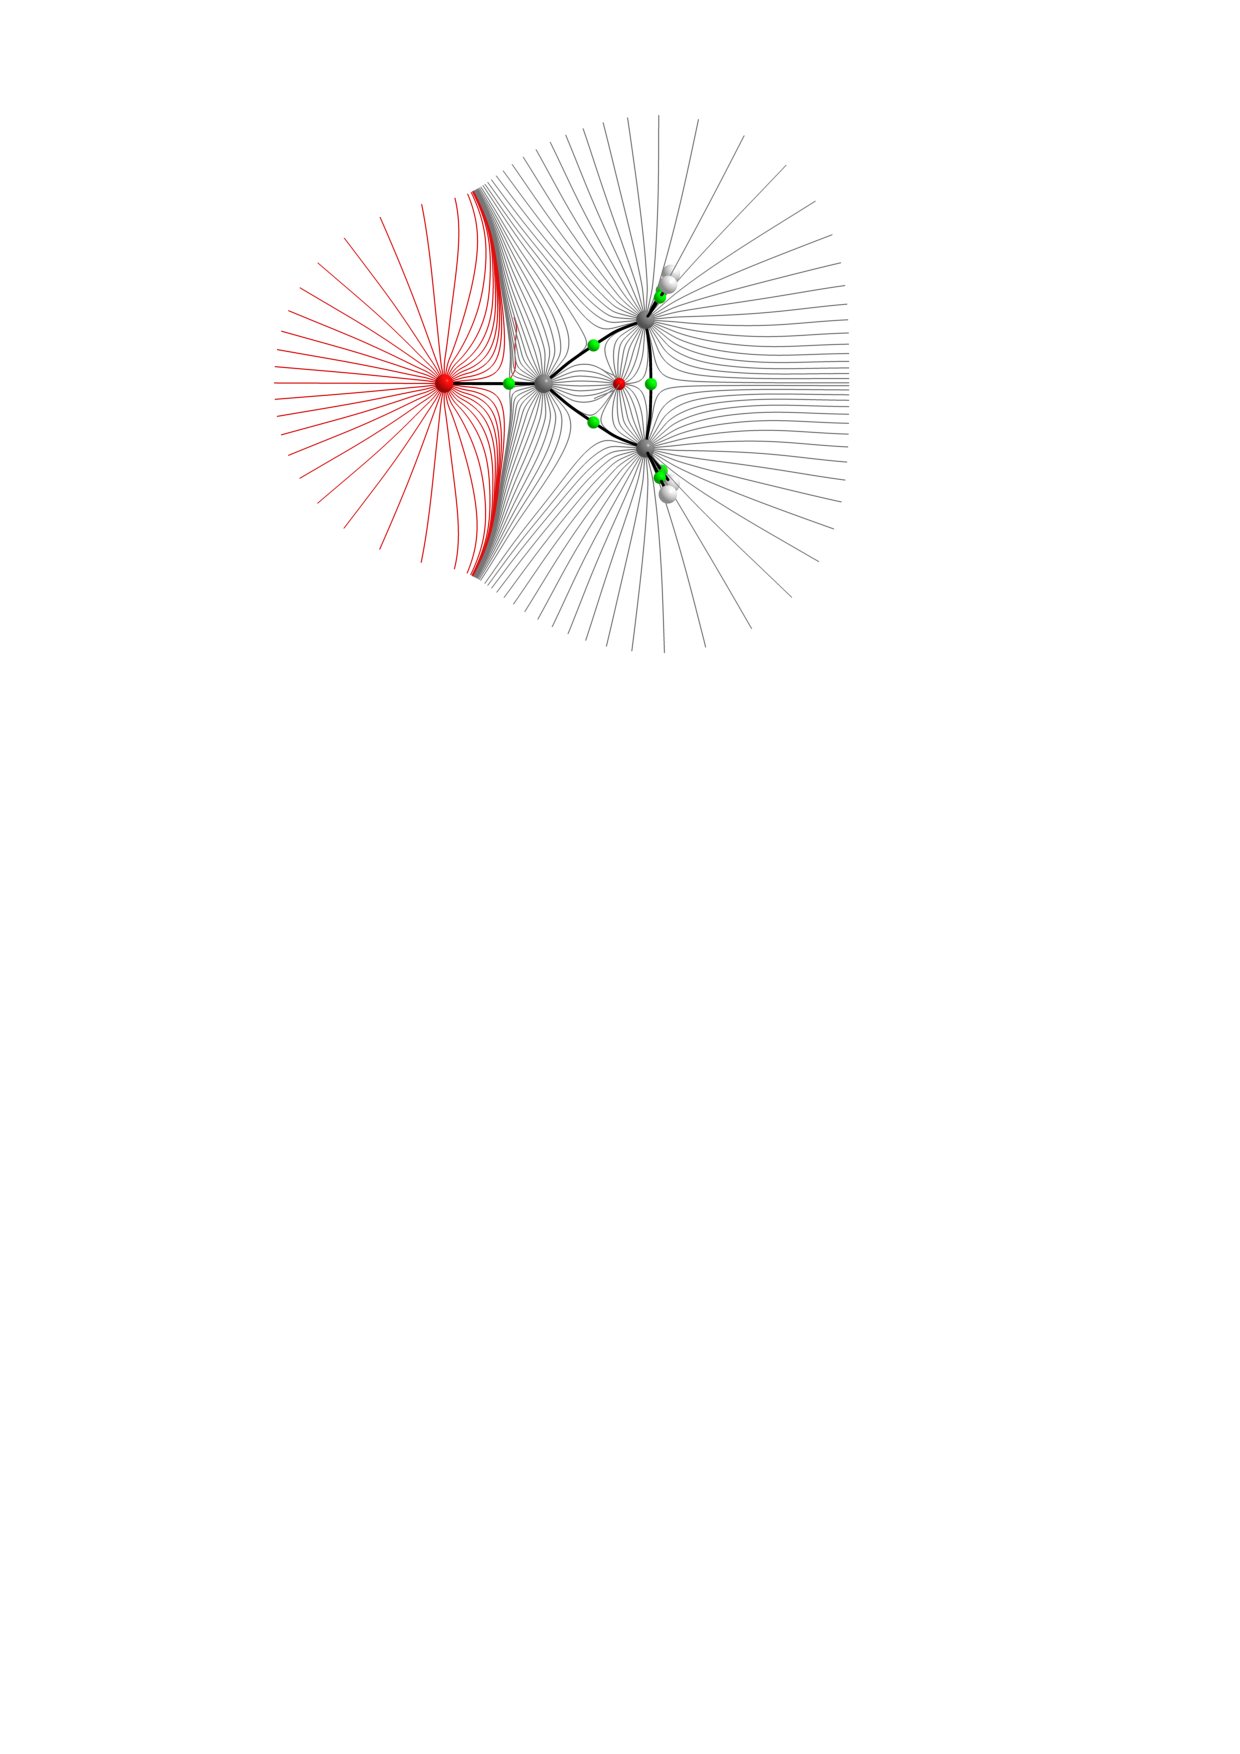
\includegraphics[width=0.5\textwidth]{3/img/flux}
  \caption{Líneas de flujo  $\nabla \rho(\mathbf{r})$ de la molécula
  de ciclopropanona (C$_3$H$_4$O).
  Dichas trayectorias delimitan regiones que pueden ser
  identificadas como átomos~\cite{todd}.}
  \label{flux}
\end{figure}

Como se muestra en la Figura \ref{flux}, los bordes de los espacios
identificados como átomos satisfacen la condición de flujo cero \ref{cero_f} y
en general, se pude hacer un análisis de máximos y mínimos de la densidad
electrónica con los valores de la Tabla \ref{PuntosCriticos}.


\subsection{Propiedades de los átomos en las moléculas}

Como se ha mencionado, las regiones $\Omega$ definidas en QTAIM se identifican
como átomos en química, y es demostrable que se cumplen los postulados de la
mecánica cuántica dentro de estas cuencas atómicas~\cite{bader}. Tomando la
condición de cero flujo, para un átomo en una molécula, llegamos a una
definición variacional de las propiedades que tiene este
subsistema~\cite{Bieglerknig1982}. Partiendo de las fronteras, identificadas
como superficies interatómicas, y de la estructura molecular se definen las
propiedades moleculares como la suma de las propiedades atómicas,
\begin{equation}
  A = \sum_{\Omega}{a_{\Omega}},
  \label{promoleculares}
\end{equation}
\noindent donde $A$ es la propiedad molecular y $a_{\Omega}$ es la misma
propiedad dentro de la cuenca $\Omega$. Todo esto basado en un principio
variacional atómico, mediante el cual se establece que si $\hat{A}$ es un
operador que equivale a la suma de operadores monoelectrónicos,
$\hat{A}=\sum\hat{a}$, entonces su valor esperado está dado por:
\begin{align}
  A(\Omega) \equiv \langle\widehat{A}\rangle_{\Omega} = \int_{\Omega}\int\cdots\int\int\cdots\int
  \left [ \frac{N}{2}\Psi_{el}^{\star}\hat{a}\Psi_{el} + (\hat{a}\Psi_{el})^{\star}\Psi_{el}\right ]
  d\omega_{1}\ldots d\omega_{N}d\mathbf{r_2}\ldots d\mathbf{r}_{N}d\mathbf{r}_{1} .
\end{align}

Esto implica que, una propiedad atómica se determina mediante la integración de
una densidad del operador asociado a dicha propiedad,
\begin{align}
  \rho_{A}(\mathbf{r})=\frac{N}{2}\int\cdots\int\int\cdots\int[
  \Psi_{el}^{\star}\hat{a}\Psi_{el} + (\hat{a}\Psi_{el})^{\star}\Psi_{el}]
  d\omega_{1}d\omega_{2}\ldots d\omega_{N}d\mathbf{r_2}\ldots d\mathbf{r}_N ,
\end{align}
y
\begin{align}
  A(\Omega)=\int_{\Omega}\rho_{A}(\mathbf{r})\mathrm{d}\mathbf{r} .
\end{align}

\subsection{Índice de deslocalización}

El índice de deslocalización, $\delta(A \leftrightarrow B)$, es una herramienta
cuantitativa dentro de QTAIM que  nos proporciona una forma de medir que tanto
se comparten electrones entre dos cuencas, que no necesariamente son primeros
vecinos. Dicho de otro modo, mide la covalencia de las interacciones. Esto ha
sugerido que el índice de deslocalización está relacionado con la covarianza de
las poblaciones electrónicas de dos cuencas, además de estar íntimamente
relacionado con las energías de intercambio-correlación.

El formalismo matemático sobre este índice está dado primeramente por el
llamado agujero de Fermi, el cual excluye a otros electrones con el mismo
espín. De forma análoga también se tiene una relación para electrones con
diferente espín, llamada agujero de Coulomb.

La imposición de la antisimetría en la función de estado electrónica, implica
que el movimiento de los electrones, que tengan la misma coordenada de espín,
está correlacionado. De la misma forma, la repulsión coulómbica impone otro
tipo de correlación. La expresión de la densidad de pares libre de correlación
electrónica se puede expresar en función de las densidades de primer orden
según la expresión: 
%Para examinar los efectos, se establece la expresión de la densidad de pares,
%en la cual los movimientos de los electrones no están correlacionados,
%
%\begin{align} \rho_2 (\mathbf{x_1 , x_2}) =
%\frac{N-1}{N}\rho(\mathbf{x_1})\rho(\mathbf{x_2}), \end{align}
%
\begin{align}
  \rho_2 (\mathbf{x_1 , x_2}) = \rho(\mathbf{x_1})\rho(\mathbf{x_2}),
\end{align}

\noindent esta expresión no toma en cuenta los efectos de la correlación
resultado de los agujeros de Fermi y Coulomb. Para tomar en cuenta dichos
efectos la expresión anterior debe ser modificada; es necesario introducir un
factor $f(\mathbf{x_1 , x_2})$ tal que:
%
%\begin{align} \rho_2 (\mathbf{x_1 , x_2}) = \frac{N-1}{N} \rho(\mathbf{x_1})
%\rho(\mathbf{x_2})[1+ f(\mathbf{x_1 , x_2})] .  \end{align}
%
\begin{align}
  \rho_2 (\mathbf{x_1 , x_2}) = \rho(\mathbf{x_1}) \rho(\mathbf{x_2})[1+ f(\mathbf{x_1 , x_2})] .
\end{align}
%La densidad de Fermi se integra a $-1$, correspondiente a la eliminación
%de la densidad de un electrón.

La correlación total de Fermi, se define como la integral de la densidad de
Fermi para cada uno de los electrones en todo el espacio y es igual a $-N$, es
decir, el número total de electrones $\alpha$ y $\beta$~\cite{Fradera1999}.  La
correlación total de Fermi es el vínculo entre la física y el modelo de Lewis.
La expresión del número promedio de pares de electrones en el átomo $A$
($D_{2}(A,A)$), o la doble integral de la densidad de pares ($\rho_{2}
(\mathbf{r}_{1}, \mathbf{r}_{2})$), se puede definir a partir del valor de la
correlación total de Fermi para dicho átomo $A$, denotado como $F(A,A)$:
%Su valor, para un átomo $A$, denotado como $F(A,A)$, puede definirse en
%términos de la expresión del número promedio de pares de electrones en el
%átomo $A$, que se obtiene de la doble integración de la densidad de pares
%$\rho_{2} (\mathbf{r}_{1}, \mathbf{r}_{2})$:
%
%\begin{align}
%D_{2}(\mathrm{A,A})=\mathrm{\int_{A}d\mathbf{r_1}\int_{A}d\mathbf{r_2}\rho(\mathbf{r_{1},r_{2}})}
%= [N(\mathrm{A})^2 + F(\mathrm{A,A})]/2 , \label{D_2_aa} \end{align}
%
\begin{align}
  D_{2}(A,A)=\mathrm{\int_{A}d\mathbf{r_1}\int_{A}d\mathbf{r_2}\rho(\mathbf{r_{1},r_{2}}) }=
  [N(A)^2 + F(A,A)]/2 ,
  \label{D_2_aa}
\end{align}

\noindent donde $N (A)$ es la población electrónica del átomo $A$. Esta
expresión muestra que el efecto neto de la correlación de Fermi es asegurar que
la densidad de pares integre al número correcto de pares formados entre un
conjunto de espines idénticos.
%Cuando A es igual a todo el espacio, $F (A, A)) =-N$, reduciendo así Número de
%pares de $\sfrac{1}{2}N^{2}$

La deslocalización de los electrones entre las cuencas atómicas $A$ y $B$ es
determinada entonces por $F(A, B)$, una cantidad que calcula la disposición en
que la densidad de Fermi en el átomo $A$ se extiende a la cuenca del átomo $B$.
De modo que, la expresión para el número promedio de pares de electrones
compartidos entre los átomos $A$ y $B$, que se obtienen al integrar las
coordenadas de un electrón de la densidad de pares sobre el átomo $A$ y las
coordenadas del otro sobre el átomo $B$, se escribe como:% en la Ecuación
\ref{D_2_ab}:
%
\begin{align}
  D_{2}(A,B)=\mathrm{\int_{A}d\mathbf{r_1}\int_{B}d\mathbf{r_2}\rho(\mathbf{r_{1},r_{2}}) }=
  [N(A)N(B) + F(A,B)]/2.
  \label{D_2_ab}
\end{align}

La misma expresión, Ecuación \ref{D_2_ab}, pude ser ahora desarrollada para
$D_{2}(B, A)$ bajo premisa de que $F(A,B)=F(B,A)$. El total de pares formados
entre $A$ y $B$ está dado por la suma de las dos poblaciones de pares. La
integración en las coordenadas de un primer electrón de la densidad de pares
sobre $A$ y del segundo sobre $A+B$ produce una expresión para la población
electrónica total del átomo $A$, definida como la suma del número de pares en
el átomo $A$ más el número de pares compartidos entre $A$ y $B$ ($D_{2} (A,A) +
D_{2} (A,B)$). La combinación de este resultado con las definiciones de
$D_{2}(A,A)$ y $D_{2}(A,B)$ llevan a la expresión para la correlación de Fermi
total obtenida de los electrones de referencia situados dentro de la cuenca
atómica de $A$,
\begin{align}
  F(A,A) +\sum_{B} F(A,B) =-N(A) ,
\end{align}

\noindent donde, en general, la suma corre para todos los átomos exceptuando a
$A$. Esto muestra que la densidad de Fermi de los electrones $N(A)$ dentro de
la cuenca de $A$ se extiende sobre los átomos restantes.

La obtención de estos índices es simple. Para obtenerlos, basta con la doble
integración, sobre el o los átomos en cuestión, de la densidad de intercambio,
que se define como la contribución a la densidad de pares que describe el
intercambio de los electrones, con el mismo espín, entre los espín-orbitales
$\phi_{i}(\mathbf{x})$. El traslape de un par de espín-orbitales sobre un átomo
$A$ como $S_{ij}(A)$ se define como: 
%
\begin{align}
  F(A,B)=F(B,A)=-\sum_i\sum_j S_{ij}(A)S_{ij}(B).
\end{align}


\section{Átomos Cuánticos Interactuantes}

Átomos Cuánticos Interactuantes (IQA por sus siglas en inglés), permite la
partición de la energía electrónica partiendo principalmente de las matrices de
densidad~\cite{blanco2005, mcweeny}. La matriz reducida de primer orden
$\rho_1(\mathbf{r}_1;\mathbf{r}_1^{\prime})$ y la densidad de pares
$\rho_2(\mathbf{r}_1,\mathbf{r}_2)$ permiten obtener la energía electrónica no
relativista bajo una aproximación Born-Oppenheimer, tal como se abordó en la
Ecuación \ref{E_b-o},
\begin{align}
  E_{\mathrm{elec}} & = \frac{1}{2} \sum_{A \neq B} \frac{Z_A Z_B}{r_{AB}} 
    + \int \widehat{h} \rho_1(\mathbf{r}_1;\mathbf{r}_1^{\prime}) \mathrm{d} \mathbf{r}_1 
    + \frac{1}{2} \int \int \frac{\rho_2(\mathbf{r}_1,\mathbf{r}_2)}{r_{12}} 
    \mathrm{d} \mathbf{r}_1 \mathrm{d} \mathbf{r}_2, \label{base}\\
  E_{\mathrm{elec}} & = V_{\mathrm{nn}}
    + \langle \widehat{T} + \widehat{V}_{\mathrm{ne}} \rangle 
    + \langle \widehat{V}_{\mathrm{ee}} \rangle,  
\end{align}
%
\noindent la parte correspondiente a la energía monoelectrónica es la suma de
la energía cinética y la atracción núcleo-electrón, es decir $\widehat{h} =
\widehat{T} + \widehat{V}_{\mathrm{ne}}$, los otros tres términos $Z_X$,
$\widehat{V}_{\mathrm{nn}}$ y $\widehat{V}_{\mathrm{ee}}$ denotan el número
atómico de $X$, la repulsión internuclear y la repulsión electrón-electrón
respectivamente.

%Para continuar con este tema es necesario, la partición del espacio en
%regiones disjuntas de Bader~\cite{bader}. El gradiente de la densidad
%electrónica, $\nabla \rho(\mathbf{r})$, forma un campo vectorial
%$\mathbf{F}:\mathbb{R}^{n} \to \mathbb{R}^{n}$ que puede ser caracterizado por
%medio de las líneas de flujo, que son  trayectorias $\sigma(t):\mathbb{R} \to
%\mathbb{R}^{n}$, definidas por la siguiente expresión.  \begin{equation}
%\sigma^{\prime} (t) =  \nabla\rho(\sigma(t)).  \end{equation}
%
%\begin{figure}
%\centering
%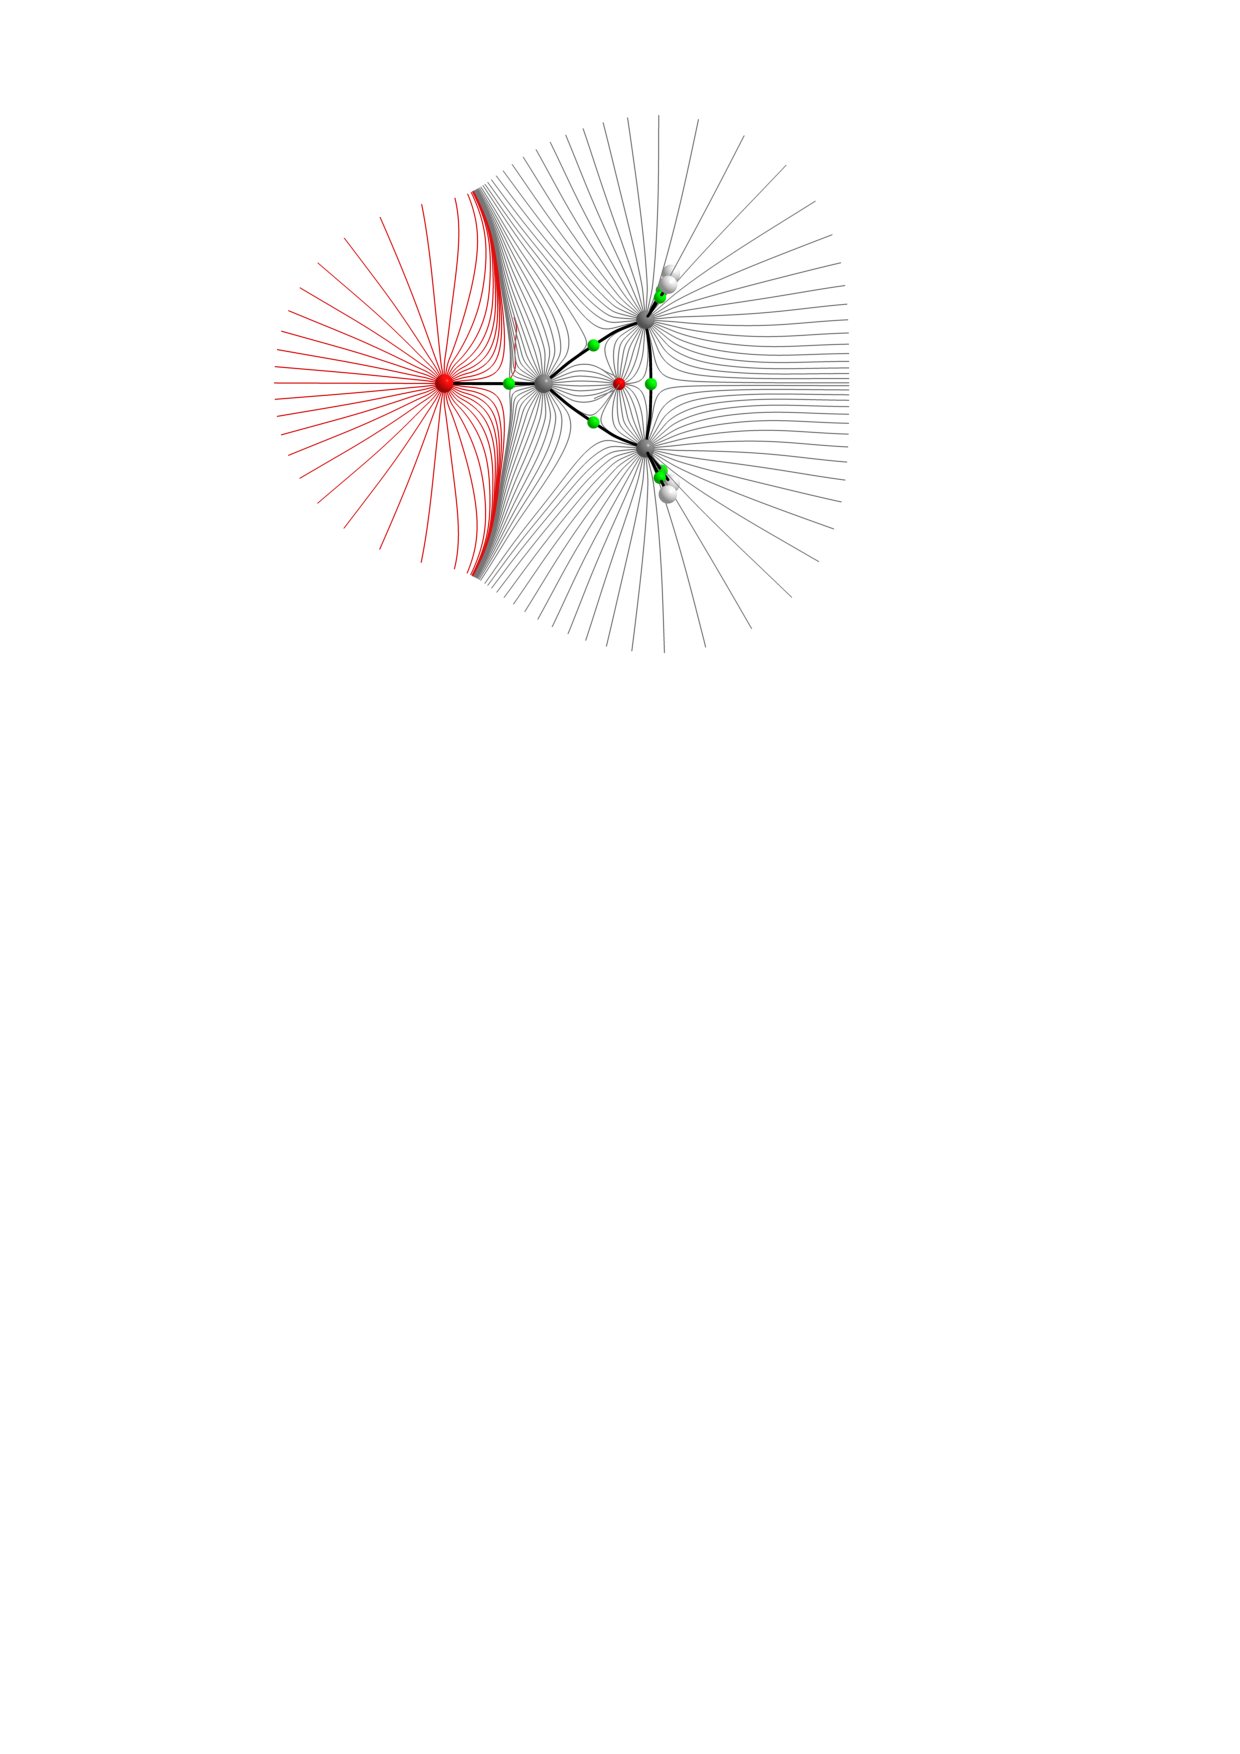
\includegraphics[width=0.5\textwidth]{3/img/flux}
%\caption{Líneas de flujo  $\nabla \rho(\mathbf{r})$ de la molécula
%de ciclopropanona (C$_3$H$_4$O).
%Dichas trayectorias delimitan regiones que pueden ser
%identificadas como átomos~\cite{todd}.}
%\label{flux}
%\end{figure}
%
%Como se muestra en la Figura \ref{flux}, los bordes de los espacios
%identificados como átomos satisfacen la condición de flujo cero \ref{cero_f} y
%en general se pude hacer un análisis con los valores de la Tabla
%\ref{PuntosCriticos}.
%
%\begin{equation}\label{ceroflujo}
%\nabla \rho(\mathbf{r})\cdot\mathbf{n} = 0. 
%\end{equation}

Después de una partición del espacio real, como la propuesta por Bader y
discutida en secciones anteriores, en la que cada región del espacio que es
delimitado por la condición de cero flujo (Ecuación \ref{cero_f}) contiene un
sólo núcleo, es decir, en el sistema no se tienen atractores no nucleares, es
posible reescribir la Ecuación \ref{base} como:
%
\footnotesize
\begin{align} 
  E_{\mathrm{elec}}  &=  \frac{1}{2} \sum_{A \neq B} \frac{Z_A Z_B}{r_{AB}} 
  -\frac{1}{2} \int \nabla^2 \rho_1(\mathbf{r}_1;
  \mathbf{r}_1^{\prime}) \mathrm{d} \mathbf{r}_1
  -\sum_A  \int \frac{Z_A \rho(\mathbf{r}_1)}{r_{1A}} \mathrm{d} \mathbf{r}_1 
  +\frac{1}{2} \int \int \frac{\rho_2(\mathbf{r}_1,
  \mathbf{r}_2)}{r_{12}} \mathrm{d} \mathbf{r}_1
  \mathrm{d} \mathbf{r}_2 \nonumber \\
      &=  \frac{1}{2} \sum_{A \neq B} \frac{Z_A Z_B}{r_{AB}} 
  -\frac{1}{2} \sum_A  \int_A   \nabla^2 \rho_1(\mathbf{r}_1;
  \mathbf{r}_1^{\prime}) \mathrm{d} \mathbf{r}_1  
  -\sum_{AB} \int_B \frac{Z_A \rho(\mathbf{r}_1)}{r_{1A}} \mathrm{d} \mathbf{r}_1
  +\frac{1}{2} \sum_{AB} \int_A \int_B \frac{\rho_2(\mathbf{r}_1,
  \mathbf{r}_2)}{r_{12}} \mathrm{d} \mathbf{r}_1 \mathrm{d} \mathbf{r}_2 \nonumber \\
      &=  \frac{1}{2} \sum_{A \neq B} V_{\mathrm{nn}}^{AB}
  +\sum_A T_A + \sum_A V_{\mathrm{ne}}^{AA}
  +\sum_{A \neq B} V_{\mathrm{ne}}^{AB} + \sum_A V_{\mathrm{ee}}^{AA} 
  +\frac{1}{2} \sum_{A \neq B} V_{\mathrm{ee}}^{AB},
\end{align}
\normalsize

%\noindent es importante notar que el orden de los superíndices y subíndices,
%debido a la referencia del núcleo o electrón de cada átomo $V_{ne}^{AB}\neq V_{ne}^{BA}$ y
%$V_{ne}^{AB}\neq V_{en}^{AB}$,
\noindent donde los términos están dados por las siguientes expresiones:
%
\begin{align}
  V_{\mathrm{nn}}^{AB} &=  \frac{Z_A Z_B}{r_{AB}}, \label{VnnAB} \\
  T_A                  &= -\frac{1}{2} \int_A \nabla^2 \rho_1 (\mathbf{r}_1;\mathbf{r}_1^{\prime})
    \mathrm{d} \mathbf{r}_1, \label{cineticaMono} \\
  V_{\mathrm{ne}}^{AB} &= - Z_A \int_B \frac{\rho(\mathbf{r}_1)}{r_{1A}} \mathrm{d}
	  \mathbf{r}_1, \label{nucleoElecMono} \\
  V_{\mathrm{ee}}^{AB} &= \frac{2 - \delta_{AB}}{2} \int_A \int_B
	  \frac{\rho_2(\mathbf{r}_1,\mathbf{r}_2)}{r_{12}} \mathrm{d} \mathbf{r}_1
	  \mathrm{d} \mathbf{r}_2. \label{elecElec2Atoms}
\end{align}


La partición IQA divide la energía electrónica en dos componentes principales:
$i$) la energía intratómica, que resulta de reagrupar los términos:
%
\begin{equation} \label{eAtomo}
E^A_{\mathrm{net}} = T^A + V_{\mathrm{ne}}^{AA} + V_{\mathrm{ee}}^{AA},
\end{equation}

\noindent y $ii$) la energía de interacción entre pares de átomos, que podemos
obtener agrupando los términos:
\begin{equation} \label{e2Atomo}
  E^{AB}_{\mathrm{int}} = V_{\mathrm{nn}}^{AB} + V_{\mathrm{ne}}^{AB}
  + V_{\mathrm{ne}}^{BA} + V_{\mathrm{ee}}^{AB}.
\end{equation}

Donde la suma de estas contribuciones (Ecuaciones \ref{eAtomo} y
\ref{e2Atomo}), tiene que regresar forzosamente la energía total del sistema
estudiado,
%
\begin{equation} \label{eElec}
E_{\mathrm{elec}} = 
  \sum_A E^A_{\mathrm{net}} + \frac{1}{2} \sum_{A \neq B} E_{\mathrm{int}}^{AB}.
\end{equation}

La Ecuación \ref{eElec} nos permite observar en la $E_{\mathrm{elec}}$ como la
suma de las contribuciones intra e interatómicas.  Adicional a la partición de
la energía electrónica que propone IQA es de suma importancia, para el
desarrollo de este trabajo, la definición de la energía interna de un
fragmento, o grupo de átomos, $\mathscr{G}$ como:
\begin{equation} \label{eG}
E^{\mathscr{G}}_{\mathrm{net}} = \sum_{A \in \mathscr{G}} E^A_{\mathrm{net}} 
    +\frac{1}{2} \sum_{A\in \mathscr{G}}
		\mathop{\sum_{B \in \mathscr{G}}}_{B \neq A} E_{\mathrm{int}}^{AB}.
\end{equation}

\noindent La energía de interacción entre dos grupos está definida por:

\begin{equation} \label{energiaGH}
E^{\mathscr{GH}}_{\mathrm{int}} = \sum_{A \in \mathscr{G}} \sum_{B \in
		 \mathscr{H}} E_{\mathrm{int}}^{AB}.
\end{equation}

Agrupar átomos permite tener una expresión para la energía de forma análoga a
la Ecuación \ref{eElec}, sólo que esta vez como función de la energía de los
grupos que forman el sistema y las energías de interacción entre los mismos,
%
\begin{equation} \label{energiaGrupos}
  E_{\mathrm{elec}} = \sum_{\mathscr{G}} E^{\mathscr{G}}_{\mathrm{net}} 
  +\frac{1}{2} \sum_{\mathscr{G} \neq \mathscr{H}} E_{\mathrm{int}}^{\mathscr{GH}}.
\end{equation}

%El separar en grupos al sistema electrónico resulta bastante útil, debido a
%que solemos definir estos grupos como moléculas, y así estudiar contribuciones
%a las interacciones intermoleculares, debido a que permite realizar una
%comparación directa de interacciones no covalentes cuando se encuentran en
%presencia o ausencia de algún otro factor, como puede ser una tercera especie.
%

La elección de los átomos, y sus interacciones, que forman en fragmento
$\mathscr{G}$ como los átomos que forman una molécula dentro de un cúmulos
molecular nos permite estudiar las energías de interacción intermoleculares, y
así, realizar una comparación directa de interacciones no covalentes y los
cambios que ocurren en dichas interacciones cuando se encuentran en presencia
de algún otro factor, como puede ser una tercera especie.

\subsection{Energía de deformación}

El concepto de \textit{energía de deformación} es de especial interés en el
desarrollo de este trabajo. Podemos entender como \textit{energía de
deformación} al cambio en la energía interna del fragmento $\mathscr{G}$ dentro
del cúmulo molecular  $\mathscr{G}\cdots\mathscr{H}\cdots\mathscr{I}\cdots$ con
respecto a la energía del fragmento aislado. Este cambio en la energía propia
del fragmento es debido a que dichos fragmentos son sacados de su geometría de
equilibro, al interactuar con los demás grupos. Si los grupos $\mathscr{G},
\mathscr{H}, \mathscr{I} \ldots$ son moléculas, la energía asociada a la
formación de un cúmulo $\mathscr{G}\cdots\mathscr{H}\cdots\mathscr{I}\cdots$
molecular se puede expresar de la siguiente manera:
%
\begin{align} 
E_{\mathrm{form}} &= E^{\mathscr{G}\cdots\mathscr{H}\cdots\mathscr{I}\cdots} 
   -\left(E^{\mathscr{G}}_{\mathrm{ais}} + E^{\mathscr{H}}_{\mathrm{ais}} + E^{\mathscr{I}}_{\mathrm{ais}}
   +\ldots \right) ,
\end{align}
\noindent sustituyendo la partición de la energía IQA, en sus componentes
intra- e intermoleculares del cúmulo
$\mathscr{G}\cdots\mathscr{H}\cdots\mathscr{I}\cdots$ (Ecuación
\ref{energiaGrupos}) en la expresión anterior y reagrupando los términos,
\begin{align}
E_{\mathrm{form}} &= \sum_{\mathscr{G}} E^{\mathscr{G}}_{\mathrm{net}} + \frac{1}{2}
    \sum_{\mathscr{G}} \sum_{\mathscr{H} \neq \mathscr{G}}
    E_{\mathrm{int}}^{\mathscr{GH}} - \left( E^{\mathscr{G}}_{\mathrm{ais}} 
   +E^{\mathscr{H}}_{\mathrm{ais}} + E^{\mathscr{I}}_{\mathrm{ais}} + \ldots \right) \nonumber \\
 &= \sum_{\mathscr{G}} (E^{\mathscr{G}}_{\mathrm{net}} - E^{\mathscr{G}}_{\mathrm{ais}}) 
   +\frac{1}{2} \sum_{\mathscr{G}} \sum_{\mathscr{H} \neq \mathscr{G}}
    E_{\mathrm{int}}^{\mathscr{GH}} ,
\end{align}
 \noindent llegamos a la definición de la energía de deformación $E^{\mathscr{G}}_{\mathrm{def}}=\sum_{\mathscr{G}} (E^{\mathscr{G}}_{\mathrm{net}} - E^{\mathscr{G}}_{\mathrm{ais}})$ de modo que, la energía de formación del cúmulo se puede reescribir como:
\begin{align}
E_{\mathrm{form}} &= \sum_{\mathscr{G}} E^{\mathscr{G}}_{\mathrm{def}}
   +\frac{1}{2} \sum_{\mathscr{G}} \sum_{\mathscr{H} \neq \mathscr{G}} 
    E_{\mathrm{int}}^{\mathscr{GH}}. \label{defInt}
\end{align} 

En la Ecuación \ref{defInt}, $E^{\mathscr{G}}_{\mathrm{ais}}$ es la energía de
la molécula aislada de $\mathscr{G}$. La energía de deformación está
relacionada con el reacomodo de la densidad electrónica en un sistema que ahora
está interactuando con algún otro sistema. El cálculo de la energía de
deformación es igual independientemente de si los sistemas estudiados son
átomos o moléculas. La Ecuación \ref{defInt} hace pensar que la generación de
un cúmulo molecular es un proceso virtual, en el que los fragmentos aislados
son sistemas ficticios a los que se les perturba al hacerlos interaccionar con
el ambiente que los rodea para, posteriormente, construir el  cúmulo. 
% donde la $\rho (\vec{r})$ y los núcleos calculados
%en los sistemas aislados, tratan de sistemas ficticios, que posteriormente se les
%perturba al hacer interactuar estos sistemas aislados con sus alrededores,
%con lo que el sistema completo da paso a deformaciones
%en los pequeños sistemas ficticios usados para la construcción del cúmulo.

%Es posible realizar una generalización sobre las interacciones a través de los
%términos clásicos (culómbico), de intercambio (Fock-Dirac) y de correlación,
%$\rho_2^\mathrm{cl}$,
%$\rho_2^\mathrm{X}$, $\rho_2^{\mathrm{corr}}$, respectivamente, de este modo
%obtener una separación de la densidad de pares:
%%
%\begin{align} \label{divRho2}
%\rho_2(\mathbf{r}_1, \mathbf{r}_2) &=
%\rho_2^{\mathrm{cl}}(\mathbf{r}_1, \mathbf{r}_2)
%+ \rho_2^{\mathrm{x}}(\mathbf{r}_1, \mathbf{r}_2)
%+ \rho_2^{\mathrm{corr}}(\mathbf{r}_1, \mathbf{r}_2)\nonumber\\
%&= \rho_2^{\mathrm{cl}}(\mathbf{r}_1, \mathbf{r}_2)
%+ \rho_2^{\mathrm{xc}}(\mathbf{r}_1, \mathbf{r}_2),
%\end{align} 
%
%\noindent en donde
%%
%\begin{align}
%\rho_2^{\mathrm{cl}}(\mathbf{r}_1, \mathbf{r}_2) &= \rho(\mathbf{r}_1)
%\rho(\mathbf{r}_2), \label{rho2C} \\
%\rho_2^{\mathrm{x}}(\mathbf{r}_1, \mathbf{r}_2)  &=  - \rho_1(\mathbf{r}_1;\mathbf{r}_2)
%\rho_1(\mathbf{r}_2;\mathbf{r}_1), \label{rho2X} \\
%\rho_2^{\mathrm{corr}}(\mathbf{r}_1, \mathbf{r}_2) &=
%\rho_2(\mathbf{r}_1, \mathbf{r}_2)
%- \rho_2^{\mathrm{cl}}(\mathbf{r}_1, \mathbf{r}_2)
%- \rho_2^{\mathrm{x}}(\mathbf{r}_1, \mathbf{r}_2), \label{rho2Corr} \\
%%\mbox{y}
%\rho_2^{\mathrm{xc}} &=  
%\rho_2^{\mathrm{x}}(\mathbf{r}_1, \mathbf{r}_2)
%+ \rho_2^{\mathrm{corr}}(\mathbf{r}_1, \mathbf{r}_2) = \rho_2(\mathbf{r}_1, \mathbf{r}_2) -
%\rho(\mathbf{r}_1) \rho(\mathbf{r}_2). \label{rho2xc}
%\end{align}
%
%La partición de $\rho_2(\mathbf{r}_1,\mathbf{r}_2)$ en la Ecuación \ref{divRho2} hace
%posible la separación de la interacción electrón-electrón entre dos átomos
%diferentes, $A \neq B$, en componentes coulómbica, de intercambio, de
%correlación y de intercambio-correlación 
%%
%\begin{align} 
%V_{\mathrm{ee}}^{AB} &= \int_A \int_B
%\frac{\rho_2(\mathbf{r}_1,\mathbf{r}_2)}{r_{12}} \mathrm{d} \mathbf{r}_1
%\mathrm{d} \mathbf{r}_2 \nonumber \\
%&= \int_A \int_B \frac{\rho_2^\mathrm{cl}(\mathbf{r}_1,\mathbf{r}_2)}{r_{12}}
%\mathrm{d}
%\mathbf{r}_1 \mathrm{d} \mathbf{r}_2 + 
%\int_A \int_B \frac{\rho_2^{xc}(\mathbf{r}_1,\mathbf{r}_2)}{r_{12}}
%\mathrm{d}
%\mathbf{r}_1 \mathrm{d} \mathbf{r}_2 \nonumber \\
%&= \int_A \int_B \frac{\rho_2^\mathrm{cl}(\mathbf{r}_1,\mathbf{r}_2)}{r_{12}}
%\mathrm{d}
%\mathbf{r}_1 \mathrm{d} \mathbf{r}_2 + 
%\int_A \int_B \frac{\rho_2^{\mathrm{x}}(\mathbf{r}_1,\mathbf{r}_2)}{r_{12}}
%\mathrm{d}
%\mathbf{r}_1 \mathrm{d} \mathbf{r}_2 +
%\int_A \int_B \frac{\rho_2^{\mathrm{corr}}(\mathbf{r}_1,\mathbf{r}_2)}{r_{12}}
%\mathrm{d}
%\mathbf{r}_1 \mathrm{d} \mathbf{r}_2 \nonumber \\
%&= V^{AB}_\mathrm{cl} + V^{AB}_{\mathrm{xc}} =
%V^{AB}_\mathrm{cl} + V^{AB}_\mathrm{x} + V^{AB}_{\mathrm{corr}}, \label{partEleEle}
%\end{align}
%
%\noindent donde
%%
%\begin{equation} \label{elementosEleEleAtomos} 
%V^{AB}_{\sigma} = \int_A \int_B \frac{\rho_2^\sigma(\mathbf{r}_1,
%\mathbf{r}_2)}{r_{12}}
%\mathrm{d} \mathbf{r}_1 \mathrm{d} \mathbf{r}_2 \hspace*{0.5cm}
%\mbox{con $\sigma = \mathrm{cl, \ x, \ corr}$ o $\mathrm{xc}$ y $A \neq B$}. \\
%\end{equation}
%
%La Ecuación \ref{partEleEle} sugiere que la energía de
%interacción entre dos átomos puede ser
%separada en dos componentes, uno clásico:
%%
%\begin{equation} \label{eleEleClas}
%V^{AB}_{\mathrm{cl}} = V^{AB}_\mathrm{k} + V^{AB}_{\mathrm{ne}} + V^{BA}_{\mathrm{ne}} + V^{AB}_{\mathrm{nn}},
%\end{equation} 
%
%\noindent y otro cuántico (intercambio-correlación), por lo que
%se puede reescribir a la energía de interacción de la Ecuación
%\ref{e2Atomo} como:
%%
%\begin{equation} \label{intClXC}
%E^{AB}_{\mathrm{int}} = V^{AB}_{\mathrm{cl}} + V^{AB}_{\mathrm{xc}}.
%\end{equation}
%
%La partición de $\rho_2(\mathbf{r}_1,\mathbf{r}_2)$ de la Ecuación
%\ref{divRho2} también puede ser utilizada para dividir la energía de 
%interacción entre dos grupos de átomos $\mathscr{G}$ y $\mathscr{H}$
%%
%\begin{equation} \label{elementosEleEleGrupos}
%V^{\mathscr{GH}}_{\sigma} = \sum_{A \in \mathscr{G}} \sum_{B \in
%		    \mathscr{H}} V^{AB}_{\sigma},
%\end{equation}
%
%\noindent donde se utilizó la Ecuación \ref{energiaGH} y $\sigma$ tiene el mismo
%significado que en la Ecuación \ref{elementosEleEleAtomos}.
%Entonces, la misma partición utilizada en la Ecuación \ref{intClXC} puede ser 
%aplicada a la interacción entre grupos:
%%
%\begin{equation} \label{intGruposClXC} 
%E^{\mathscr{GH}}_{\mathrm{int}} = V^{\mathscr{GH}}_{\mathrm{cl}} +
%V^{\mathscr{GH}}_{\mathrm{xc}},
%\end{equation}
%
%\noindent en la cual la interacción clásica es 
%%
%\begin{equation} \label{eleEleClasGrupo}
%V^{\mathscr{GH}}_{\mathrm{cl}} = V^{\mathscr{GH}}_\mathrm{k} + V^{\mathscr{GH}}_{\mathrm{ne}} +
%V^{\mathscr{HG}}_{\mathrm{ne}} + V^{\mathscr{GH}}_{\mathrm{nn}},
%\end{equation} 
%
%\noindent y $V^{\mathscr{GH}}_{\mathrm{xc}}$ está dada por la
%Ecuación \ref{elementosEleEleGrupos} cuando $\sigma = \mathrm{xc}$.
%
%Finalmente, es importante notar que los componentes de la energía de
%repulsión electrónica dentro de un átomo también se pueden obtener
%mediante una expresión muy similar a la ecuación
%\ref{elementosEleEleAtomos}. Sin embargo, se debe tener
%cuidado de considerar el factor de $\sfrac{1}{2}$ en las expresiones \ref{elecElec2Atoms}, 
%\ref{partEleEle} y \ref{elementosEleEleAtomos}.

\subsection{Energía de interacción}

Es posible separar la densidad de pares en una suma de los términos: $i$)
clásico o coulómbico ($\rho_2^\mathrm{cou}$), $ii$) de intercambio o de
Fock-Dirac ($\rho_2^\mathrm{x}$) y $iii$) de correlación
($\rho_2^\mathrm{corr}$).
%
\begin{align} \label{divRho2}
  \rho_2(\mathbf{r}_1, \mathbf{r}_2) &=
  \rho_2^{\mathrm{cou}}(\mathbf{r}_1, \mathbf{r}_2)
  + \rho_2^{\mathrm{x}}(\mathbf{r}_1, \mathbf{r}_2)
  + \rho_2^{\mathrm{corr}}(\mathbf{r}_1, \mathbf{r}_2)\nonumber\\
  &= \rho_2^{\mathrm{cou}}(\mathbf{r}_1, \mathbf{r}_2)
  + \rho_2^{\mathrm{xc}}(\mathbf{r}_1, \mathbf{r}_2),
\end{align} 

\noindent donde:
%
\begin{align}
  \rho_2^{\mathrm{cou}}(\mathbf{r}_1, \mathbf{r}_2) &= \rho(\mathbf{r}_1)
  \rho(\mathbf{r}_2), \label{rho2C} \\
  \rho_2^{\mathrm{x}}(\mathbf{r}_1, \mathbf{r}_2)  &=  - \rho_1(\mathbf{r}_1;\mathbf{r}_2)
  \rho_1(\mathbf{r}_2;\mathbf{r}_1), \label{rho2X} \\
  \rho_2^{\mathrm{corr}}(\mathbf{r}_1, \mathbf{r}_2) &=
  \rho_2(\mathbf{r}_1, \mathbf{r}_2)
    - \rho_2^{\mathrm{cou}}(\mathbf{r}_1, \mathbf{r}_2)
    - \rho_2^{\mathrm{x}}(\mathbf{r}_1, \mathbf{r}_2), \label{rho2Corr} \\
  \rho_2^{\mathrm{xc}} &=  
  \rho_2^{\mathrm{x}}(\mathbf{r}_1, \mathbf{r}_2)
    + \rho_2^{\mathrm{corr}}(\mathbf{r}_1, \mathbf{r}_2) = \rho_2(\mathbf{r}_1, \mathbf{r}_2) -
  \rho(\mathbf{r}_1) \rho(\mathbf{r}_2).
  \label{rho2xc}
\end{align}

La partición de $\rho_2(\mathbf{r}_1,\mathbf{r}_2)$ en la Ecuación
\ref{divRho2} hace posible la separación de la interacción electrón-electrón
entre dos átomos diferentes, $A$  y $B$, en componentes coulómbica y de
intercambio-correlación, 
%
\begin{align} 
  V_{\mathrm{ee}}^{AB} &= \int_A \int_B
  \frac{\rho_2(\mathbf{r}_1,\mathbf{r}_2)}{r_{12}} \mathrm{d} \mathbf{r}_1 \mathrm{d} \mathbf{r}_2 \nonumber \\
  &= \int_A \int_B \frac{\rho_2^\mathrm{cou}(\mathbf{r}_1,\mathbf{r}_2)}{r_{12}}
    \mathrm{d}
    \mathbf{r}_1 \mathrm{d} \mathbf{r}_2 + 
    \int_A \int_B \frac{\rho_2^{\mathrm{xc}}(\mathbf{r}_1,\mathbf{r}_2)}{r_{12}}
    \mathrm{d}
    \mathbf{r}_1 \mathrm{d} \mathbf{r}_2 \nonumber \\
  &= \int_A \int_B \frac{\rho_2^\mathrm{cou}(\mathbf{r}_1,\mathbf{r}_2)}{r_{12}}
    \mathrm{d}
    \mathbf{r}_1 \mathrm{d} \mathbf{r}_2 + 
    \int_A \int_B \frac{\rho_2^{\mathrm{x}}(\mathbf{r}_1,\mathbf{r}_2)}{r_{12}}
    \mathrm{d}
    \mathbf{r}_1 \mathrm{d} \mathbf{r}_2 +
    \int_A \int_B \frac{\rho_2^{\mathrm{corr}}(\mathbf{r}_1,\mathbf{r}_2)}{r_{12}}
    \mathrm{d}
    \mathbf{r}_1 \mathrm{d} \mathbf{r}_2 \nonumber \\
  &= V^{AB}_\mathrm{cou} + V^{AB}_{\mathrm{xc}} =
    V^{AB}_\mathrm{cou} + V^{AB}_\mathrm{x} + V^{AB}_{\mathrm{corr}}, \label{partEleEle}
\end{align}

\noindent donde:
%
\begin{equation} \label{elementosEleEleAtomos} 
  V^{AB}_{\sigma} = \int_A \int_B \frac{\rho_2^\sigma(\mathbf{r}_1,
  \mathbf{r}_2)}{r_{12}}
  \mathrm{d} \mathbf{r}_1 \mathrm{d} \mathbf{r}_2 , \hspace*{0.5cm}
  \mbox{con $\sigma = \mathrm{cou, \ x, \ corr}$ o $\mathrm{xc}$ y $A \neq B$}. \\
\end{equation}

La Ecuación \ref{partEleEle} sugiere que la energía de interacción entre dos
átomos puede ser separada en dos componentes, uno clásico:
%
\begin{equation} \label{eleEleClas}
V^{AB}_{\mathrm{cl}} = V^{AB}_\mathrm{cou} + V^{AB}_{\mathrm{ne}} + V^{BA}_{\mathrm{ne}} + V^{AB}_{\mathrm{nn}},
\end{equation} 

\noindent y otro cuántico (intercambio-correlación $V_{\mathrm{xc}}^{AB}$), por
lo que se puede reescribir a la energía de interacción (Ecuación
\ref{e2Atomo}) como:
%
\begin{equation} \label{intClXC}
E^{AB}_{\mathrm{int}} = V^{AB}_{\mathrm{cl}} + V^{AB}_{\mathrm{xc}}.
\end{equation}

%La partición de $\rho_2(\mathbf{r}_1,\mathbf{r}_2)$ de la Ecuación
%\ref{divRho2} también puede ser utilizada para dividir la energía de 
%interacción entre dos grupos de átomos $\mathscr{G}$ y $\mathscr{H}$
%%
%\begin{equation} \label{elementosEleEleGrupos}
%V^{\mathscr{GH}}_{\sigma} = \sum_{A \in \mathscr{G}} \sum_{B \in
%		    \mathscr{H}} V^{AB}_{\sigma},
%\end{equation}
%
%\noindent donde se utilizó la Ecuación \ref{energiaGH} y $\sigma$ tiene el mismo
%significado que en la Ecuación \ref{elementosEleEleAtomos}.
%Entonces, la misma partición utilizada en la Ecuación \ref{intClXC} puede ser 
%aplicada a la interacción entre grupos:
%%
%\begin{equation} \label{intGruposClXC} 
%E^{\mathscr{GH}}_{\mathrm{int}} = V^{\mathscr{GH}}_{\mathrm{cl}} +
%V^{\mathscr{GH}}_{\mathrm{xc}},
%\end{equation}
%
%\noindent en la cual la interacción clásica es 
%%
%\begin{equation} \label{eleEleClasGrupo}
%V^{\mathscr{GH}}_{\mathrm{cl}} = V^{\mathscr{GH}}_\mathrm{k} + V^{\mathscr{GH}}_{\mathrm{ne}} +
%V^{\mathscr{HG}}_{\mathrm{ne}} + V^{\mathscr{GH}}_{\mathrm{nn}},
%\end{equation} 
%
%\noindent y $V^{\mathscr{GH}}_{\mathrm{xc}}$ está dada por la
%Ecuación \ref{elementosEleEleGrupos} cuando $\sigma = \mathrm{xc}$.

Los términos $V_{\mathrm{cl}}^{\mathrm{AB}}$ y $V_{\mathrm{xc}}^{\mathrm{AB}}$
son comúnmente identificados como componentes iónicos y covalentes,
respectivamente, de la energía de interacción entre los átomos $A$ y $B$. El
concepto de interacción entre átomos puede ser extrapolado a grupos de átomos,
generalmente moléculas, $\mathscr{G}$, $\mathscr{H}$, $\mathscr{I}$, \ldots
dentro un sistema,

\begin{align}
  E = \displaystyle\sum_{\mathscr{G}}E_{\mathrm{net}}^{\mathscr{G}} + 
      \displaystyle\frac{1}{2}\displaystyle\sum_{\mathscr{G}}\displaystyle\sum_{\mathscr{G\neq H}}E_{\mathrm{int}}^{\mathscr{GH}}, 
\end{align}

\noindent en donde:

\begin{align} \label{e_net}
E_{\mathrm{net}}^{\mathscr{G}} &= \displaystyle\sum_{\mathrm{A}\in\mathscr{G}}E_{\mathrm{net}}^{\mathrm{A}} +
                                  \displaystyle\frac{1}{2}\displaystyle\sum_{\mathrm{A}\in\mathscr{G}}
                                  \displaystyle\sum_{\substack{\mathrm{B}\in\mathscr{G} \\ \mathrm{B}\neq \mathrm{A}}}E_{\mathrm{int}}^{\mathrm{AB}},
\end{align}

\noindent y

\begin{align}
E_{\mathrm{int}}^{\mathscr{GH}} &= \displaystyle\sum_{\mathrm{A}\in\mathscr{G}}\displaystyle\sum_{\mathrm{B}\in\mathscr{H}}E_{\mathrm{int}}^{\mathrm{AB}}.
\end{align}

Por lo cual es posible representar el cambio de la energía en términos de la
energía asociada a la formación del cúmulo molecular, $ \mathscr{G} +
\mathscr{H} + \mathscr{I} + \cdots$ \ce{<=>}
$\mathscr{G}\cdots\mathscr{H}\cdots\mathscr{I}\cdots $, como la suma:

\begin{align}
\Delta E = \sum_{\mathscr{G}} E_{\mathrm{def}}^{\mathscr{G}} +
           \sum_{\mathscr{G}} \sum_{\mathscr{G>H}} E_{\mathrm{int}}^{\mathscr{GH}}, 
\label{iqa_g}
\end{align}

\noindent donde $E_{\mathrm{def}}^{\mathscr{G}}$ denota la energía de
deformación del grupo $\mathscr{G}$, la diferencia en la energía entre $i$)
$\mathscr{G}$ en el cúmulo molecular (calculada con la Ecuación \ref{e_net}) y
$ii$) $\mathscr{G}$ aislado de su geometría de equilibrio~\cite{blanco2005}.
Podemos reescribir la Ecuación \ref{iqa_g} como una suma de
pares~\cite{Toche2016},
%
\begin{align}
\Delta E &= \displaystyle\sum_{\mathscr{G}}\displaystyle\sum_{\mathscr{G>H}}\left(E_{\mathrm{int}}^{\mathscr{GH}} + 
           \left(\displaystyle\frac{E_{\mathrm{int}}^{\mathscr{GH}}}{\displaystyle\sum_{\mathscr{J\neq
           G}}E_{\mathrm{int}}^{\mathscr{JG}}}\right)E_{\mathrm{def}}^{\mathscr{G}}
           + \left(\displaystyle\frac{E_{\mathrm{int}}^{\mathscr{GH}}}{\displaystyle\sum_{\mathscr{J\neq
           H}}E_{\mathrm{int}}^{\mathscr{JH}}}\right)E_{\mathrm{def}}^{\mathscr{H}}\right) \nonumber \\
         &=\displaystyle\sum_{\mathscr{G}}\displaystyle\sum_{\mathscr{G>H}}E_{\mathrm{int}}^{\mathscr{GH'}},
  \label{eintprima}
\end{align}

\noindent en donde $E_{\text{int}}^{\mathscr{GH'}}$ incluye
$E_{\mathrm{int}}^{\mathscr{GH}}$ y una fracción de
$E_{\mathrm{def}}^{\mathscr{G}}$ y $E_{\mathrm{def}}^{\mathscr{H}}$.  A su vez,
es posible proponer una partición de energía electrónica
$E_{\mathrm{int}}^{\mathscr{GH'}}$ (Ecuación \ref{eintprima}), en términos de
los componentes clásicos y de intercambio-correlación,
%
\begin{align}
\Delta E &= \displaystyle\sum_{\mathscr{G}}\displaystyle\sum_{\mathscr{G>H}}\left(E_{\mathrm{xc}}^{\mathscr{GH}} 
           + E_{\mathrm{cl}}^{\mathscr{GH}}\right)\left( 1 + \left(\displaystyle\frac{1}{\displaystyle\sum_{\mathscr{J\neq
           G}}E_{\mathrm{int}}^{\mathscr{JG}}}\right)E_{\mathrm{def}}^{\mathscr{G}}
           + \left(\displaystyle\frac{1}{\displaystyle\sum_{\mathscr{J\neq
           H}}E_{\mathrm{int}}^{\mathscr{JH}}}\right)E_{\mathrm{def}}^{\mathscr{H}}\right) \nonumber \\
         &= \displaystyle\sum_{\mathscr{G}}\displaystyle\sum_{\mathscr{G>H}}\left(E_{\mathrm{xc}}^{\mathscr{GH'}}
           + E_{\mathrm{cl}}^{\mathscr{GH'}}\right).
  \label{eint_cl_xc_prima}
\end{align}

\section{Detalles Computacionales}

Las optimizaciones de los 16 cúmulos de agua $\mathrm{(H_2O)_n}$ $\mathrm{n=6,
...,17}$, mostrados en la Figura \ref{cumulos}, se realizaron con el método
M06-2X/6-311++G(d,p)~\cite{Zhao2006,McLean1980}, usando el programa
{\sc{Gaussian09}}~\cite{g09}. La elección del funcional y la base orbital está
basada en estudio realizado por Jiménez Gravalos y colaboradores
\citenum{JimenezGravalos2019} en el que se sugiere que dicho método reproduce
adecuadamente el comportamiento cooperativo y anticooperativo descrito por las
funciones de estado correlacionadas a cúmulos de agua a un costo computacional
moderado~\cite{JimenezGravalos2019}.

Los análisis de las particiones del espacio real de QTAIM y de la energía
electrónica de IQA se llevaron acabo como están
implementadas~\cite{Maxwell2016,Francisco2016} en el código
{\sc{AIMAll}}~\cite{aimall} con densidades obtenidas del programa
{\sc{Gaussian09}}~\cite{g09} y el mismo método descrito para la optimización de
geometrías.  La lectura de las salidas y el álgebra pertinente fue realizado
por medio de scripts escritos en Perl~\cite{wall2000programming}.  Las
representaciones pictóricas de los resultados se realizaron con ayuda de
{\sc{GausView}}~\cite{g09}, Matplotlib~\cite{Hunter2007} y estilizadas con
GIMP~\cite{gimp}.
%e INKSCAPE~\cite{Inkscape}.
